\documentclass[a4paper,11pt]{scrreprt}

\usepackage[komastyle,automark]{scrpage2}
%\usepackage{german}
\usepackage[latin1]{inputenc}
\usepackage{graphicx}
\usepackage[a4paper,left=2.5cm,top=2.5cm,bottom=2.5cm,includeheadfoot,width=16cm]{geometry}

\setlength{\parindent}{0em}
\setlength{\parskip}{1.5ex plus0.5ex minus0.5ex}
%\setlength{\textheight}{217mm}
%\setlength{\textwidth}{170mm}

\renewcommand{\captionformat}{~---~}
\setcapindent{0mm}
\addtokomafont{caption}{\small}
\setkomafont{captionlabel}{\sffamily \bfseries}

\setlength{\tabcolsep}{3mm}
\renewcommand{\arraystretch}{1.2}


%\documentclass[11pt]{report}

%\usepackage[utf8]{inputenc}
\usepackage{ngerman}
\usepackage{ae}
\usepackage{amsmath}
\usepackage{listings}
\usepackage[german]{varioref}



\usepackage{graphicx}
\usepackage{epstopdf}

%\usepackage[dvips]{graphicx}
\DeclareGraphicsExtensions{.eps,.gif}

\usepackage{nonfloat} % Einf�gen von Bildern ohne Float (\figcaption)
\usepackage[percent]{overpic}
\usepackage{overpic}


\usepackage{picins}  % frameenv
\usepackage{wrapfig} % umfliessende Bilder

\setcounter{secnumdepth}{2} \setcounter{tocdepth}{2} 
\renewcommand{\topfraction}{.99}
\renewcommand{\bottomfraction}{.3}
\renewcommand{\textfraction}{0.00001}

\bibliographystyle{alphadin} 


\newenvironment{compactitemize}
    {
    \begin{list}{-}{%
        \setlength{\itemsep}{0pt}%
    }}
    {\end{list}}

\clubpenalty=15000%
\widowpenalty=10000%
\displaywidowpenalty=10000%


\begin{document}

% Deckblatt

\begin{titlepage}

  \begin{center}
     \LARGE \bf
     Zielgerichtete Anpassung eines WCMS \\an die Anforderungen einer \\Kommunikationsplattform - Eine Fallstudie im Bereich der Lehrerbildung
      
\normalsize \mdseries
    \vspace*{2cm}
    { \large \bf Bachelorarbeit}

    \begin{center}\bf
    im Studiengang Software Systems Science\\
    in der Fakult�t Wirtschaftsinformatik und Angewandte
    Informatik\\
    der\\
    Otto-Friedrich-Universit�t Bamberg
    \end{center}
    \vspace{1cm}

     vorgelegt von \\
    \vspace*{0.7cm}
    {\Large \bf Felix Gellner} \\
    \vspace*{0.7cm}

    \vspace{5cm}

    angefertigt am

    \vspace{0.1cm}

    {
      Lehrstuhl f�r Medieninformatik\\

      Universit�t Bamberg \\
      }

    \vspace{1cm}

    Pr�fer: Prof. Dr. Andreas Henrich\\

    \vspace{1cm}

    Beginn der Arbeit: 09.04.2016 \\
    Abgabe der Arbeit: 21.07.2016

  \end{center}
\end{titlepage}


\pagenumbering{roman}%

%Inhaltsverzeichnis
\tableofcontents%
\newpage
\pagestyle{headings}%
\pagenumbering{arabic}%
\setcounter{page}{1}
\parskip1.5ex


\chapter{Einleitung}

Moderne Webanwendungen und Plattformen beinhalten heutzutage weitaus mehr als die M�glichkeit statische Informationen anzuzeigen. Mit dem Aufkommen des Web 2.0 hat das Internet einen gewaltigen Sprung gemacht und ein weiteres Mal die Welt ver�ndert. Und wenn es auch f�r einige Leute immer noch Neuland ist, sind die Vorz�ge des Internets inzwischen auch bei den traditionelleren Institutionen, wie dem deutschen Staat, mit hohem Ansehen vertreten. So kommt es, dass der Staat Deutschland 2013 ein massives Projekt zur Verbesserung der Bildung ins Leben gerufen hat, das im Namen des WegE Projekts der Otto-Friedrich Universit�t Bamberg eine staatlich gef�rderte Online-Pr�senz dazugewinnt. Um solche Webpr�senzen umzusetzen verl�sst man sich heutzutage auf ein F�llhorn von Technologien, welche versprechen, die Entwicklung, der zunehmend komplexen Systeme, zu erleichtern. Besonders der dynamische Charakter moderner Webseiten erfordert eine andere Herangehensweise als die urspr�nglich statischen HTML-Seiten. Diese und noch viele andere Aufgaben �bernehmen Web Content Management Systeme f�r uns. Ist man an dieser Erkenntnis angelangt, bedarf es nur noch der Entscheidung f�r eines der �ber 1200 verf�gbaren Web Content Management Systeme. F�r diese Entscheidung sollte wiederum vorher klar sein, welche genauen Ziele ein Projekt verfolgt. Erst nach all diesen Schritten und einer groben Einarbeitung in die gew�hlten Technologien l�sst sich eine fundierte Zeit- und Kostenabsch�tzung erzeugen, geschweige denn das Projekt umsetzen. Genau diese, und weitere verwandte Dinge, werden in der folgenden Arbeit in einem allgemeinen Licht, und im Bezug auf das WegE Projekt der Universit�t Bamberg, behandelt.

\section{Das WegE Projekt}

\begin{figure}[hbtp]
	\centering
	
\includegraphics[scale=1]{abb/wege_logo.png}
	\caption{WegE Logo}
\end{figure}

Das WegE Projekt der Universit�t Bamberg ist ein Teil der 'Qualit�tsoffensive Lehrerbildung'. Mit dieser Offensive wollen Bund und L�nder die Kompetenzen der Lehrer st�rken. WegE steht f�r 'Wegweisende Lehrerbildung' und hat als Hauptziel die Entwicklung reflexiver Kommunikationsprozesse, vor Allem in Bamberg. Die fachliche Zusammenarbeit zwischen Wissenschaftlern und Lehrern, sowie Lehramtsstudenten soll verbessert werden. Die Lehrerbildung an den fachlichen St�rken der Universit�t Bamberg wird profiliert, die Zusammenarbeit von Fachwissenschaften und Schulen wird gest�rkt, die Fortbildungsangebote werden ausgebaut und das Gesamtprojekt wird f�r zuk�nftige Vorhaben aufw�ndig evaluiert. All dies f�hrt zu dem simpleren, indirekten Ziel der Verbesserung der Lehrer und somit auch der Schulbildung. Da sich das Projekt aktuell in Entwicklung befindet, k�nnen Ziele sich zum Zeitpunkt der Ver�ffentlichung dieser Arbeit leicht ver�ndert haben. \cite{wege}

\begin{figure}[hbtp]
	\centering
	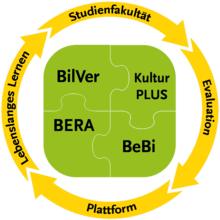
\includegraphics[scale=0.5]{abb/wege.png}
	\caption{Die Bestandteile des WegE Projekts}
\end{figure}

Das WegE Projekt besteht im Wesentlichen aus vier einzelnen Projektvorhaben:
\begin{description}
	\item{\emph{KulturPLUS}}
	
	Die Organisation KulturPLUS wird sich der Vernetzung geistes- und kulturwissenschaftlicher Perspektiven widmen. Dieses Vorhaben geht von den Fakult�ten Geistes- und Kulturwissenschaften und Humanwissenschaften, genauer der Evangelischen Theologie, aus. Durch verschiedene M�glichkeiten soll Lehramtsstudenten die Kompetenz zum Umgang mit den Herausforderungen der kulturellen Vielfalt bez�glich sprachlicher, historischer, geographischer und religi�ser Kontexte, beigebracht werden. Die konkrete Umsetzung dieser Ziele ist durch verschiedene Optionen vorgesehen. Darunter ein Wahlpflichtkurs namens \textit{KulturPLUS-Modul}, die �berarbeitung von Schulpraktika und die Ver�ffentlichung fachwissenschaftlicher Ergebnisse auf der WegE Plattform.\footnote{https://www.uni-bamberg.de/wege/kulturplus/}

	\item{\emph{BilVer}}

	BilVer (\textsc{Bil}dungswissenschaft im \textsc{Ver}bund) k�mmert sich um die fallbezogene Vernetzung der bildungswissenschaftlichen Ausbildungsstelle. \textquotedblleft Im Mittelpunkt des Projektvorhabens stehen dabei vor allem die inhaltliche Abstimmung zwischen einzelnen F�chern, die St�rkung des Professions- und Schulbezugs sowie der darauf bezogene Ausbau fall- und themenbezogener Lehr-, Lern- und Pr�fungsformate.\textquotedblright\cite{wege}. Konkret soll der bildungswissenschaftliche Bereich der Lehramtstudieng�nge an der Universit�t Bamberg durch eine bessere Kommunikation zwischen Ausbildungsinhalten verschiedener Disziplinen, st�rkere Berufsbez�ge und innovativere Lehr- und Pr�fungsformate, verbessert werden.\footnote{https://www.uni-bamberg.de/wege/bilver/}

\item{\emph{BERA}}

BERA (\textsc{Bera}tung im schulischen Kontext) hat als Ziel den Aufbau eines Kompetenzzentrums in Bamberg. Dessen Aufgabe wird die St�rkung der beratungsbezogenen Professionsanteile im Studium und die Kooperation mit den Schulen der Region sein. Als zweiter Punkt wird ein Querschnittsmodul erstellt, welches Lehramtsstudenten Beratungskompetenz im schulischen Kontext lehren soll. Im Rahmen dieses Moduls werden im geplanten Beratungszentrum von BERA, praktische Verantstaltungen abgehalten, welche die Durchf�hrung verschiedener Beratungsformate zeigen. Die Bekanntmachung solcher Verantstaltungen soll auch �ber die WegE Plattform laufen.\footnote{https://www.uni-bamberg.de/wege/bera/}

\item{\emph{BeBi}}

BeBi (\textsc{Be}rufliche \textsc{Bi}ldung) wird sich mit der Profilierung der Studieng�nge Wirtschaftsp�dagogik und Berufliche Bildung/Fachrichtung Sozialp�dagogik, besch�ftigen. Im Studiengang Berufliche Bildung werden eine st�rkere inhaltliche Vernetzung der beteiligten F�cher, angestrebt. In Folge dessen wird im beteiligten Fach Psychologie ein Wahlpflichtbereich erweitert. Dieser tr�gt den Namen Fr�he Bildung und Entwicklung und soll mehr berufsbezogene, praktische Module enthalten. Im Studiengang Wirtschaftsp�dagogik wird ebenfalls eine Erweiterung des Lehrangebots durch das Erstellen neuer Module im sozialp�dagogischen Bereich, angestrebt.\footnote{https://www.uni-bamberg.de/wege/bebi/}

\end{description}

Unterst�tzt wird das WegE Projekt von vier weiteren Institutionen, eine davon, Strukturma�nahme 3: Bildungs- und Internetplattform, hat die Funktion, die Kommunikation und Kooperation zwischen allen Projekten zu gew�hren und das Engagement von au�enstehenden Personen zu f�rdern. Im Mittelpunkt steht hier also die Internetplattform des Projekts WegE. Dies ist die Strukturma�nahme, welche im idealen Fall von den Ergebnissen dieser Bachelorarbeit am Meisten profitiert. Die genauen Ziele der Strukturma�nahme 3, welche in dieser Arbeit untersucht werden sollen, sind in Kapitel 3.3 gelistet.\footnote{https://www.uni-bamberg.de/wege/plattform/}

In die Qualit�tsoffensive Lehrerbildung investieren Bund und L�nder bis 2023 insgesamt eine halbe Milliarde Euro. 3,35 Millionen Euro flie�en davon in das WegE Projekt der Universit�t Bamberg. Der Zeitraum f�r die F�rderung des WegE Projekts ist weniger lang. Dieser begann am 01.01.2016 und wird bis zum 30.06.2019 bestehen bleiben.

\section{Zielsetzung und Vorgehensweise}

Das haupts�chliche Ziel dieser Arbeit wird aus dem konkreten Projekt der wegweisenden Lehrerbildung motiviert und ist die Analyse einer Liste spezifischer Requirements auf ihre Machbarkeit und den zu erwartenden Aufwand. Grunds�tzlich wird jedoch ein allgemeinerer Ton angeschlagen, um so eine Relevanz f�r technisch �hnliche Projekte zu erreichen. Es geht um die Planung und Umsetzung von web-basierten Plattformen mit Kommunikationsaspekt und einer merklichen Gr��e. 

In den folgenden Kapiteln werden zun�chst die Anforderungen an das System behandelt. Je gr��er ein Projekt, desto wichtiger die Planungsphase.
Kapitel \ref{fig:SoftwareProcessModels} gibt eine Struktur vor, wie solche Web Content Management Projekte geplant und entwickelt werden k�nnen. \\
Ein wichtiger Aspekt der Planung von Software sind Anforderungen (engl. Requirements). Es wird betrachtet, was die Requirements einer web-basierten Plattform sind und wie diese Anforderungen festgehalten und validiert werden. Die spezifisch zu untersuchenden Requirements der WegE Plattform wurden haupts�chlich in mehreren Meetings mit den Vertretern aller beteiligten Teilprojekte erhoben. Der Prozess wird in Kapitel 2 erkl�rt. Anschlie�end werden die M�glichkeiten der technischen Umsetzung verglichen. Konkret wird der Vergleich verschiedener Content Management Systeme hinsichtlich der Anforderungen gezogen. Im Hauptteil wird die technische Umsetzung der einzelnen, gesammelten Anforderungen im Bezug auf ein Content Management System, genau gepr�ft, getestet und anhand sinnvoller Kriterien evaluiert. Die technische Umsetzung einzelner Anforderungen geschieht oft mit Erweiterungen zu einem CMS. Hierzu wird die Eignung bereits bestehender Erweiterungen untersucht und passende Erweiterungen zu Testzwecken implementiert. Nach der Analyse der Requirements werden, zum Ende hin, die angestrebten Features der WegE Plattform auf ihren Mehrwert untersucht und vor Allem ihre Machbarkeit evaluiert.
      
\chapter{Begriffskl�rungen}

Zum vollen Verst�ndnis der Arbeit werden grundlegende Kenntnisse des Software Engineering und der Web Technologien vorausgesetzt. Weitere essentielle Begrifflichkeiten und Technologien werden nun erkl�rt.

\section{CMS und WCMS}

Ein Content Management System (Abk. CMS), oder auf Deutsch Inhaltsverwaltungssystem, ist eine Software, die bei der Erstellung, Pflege und Planung von Content helfen kann. Vor Allem dann, wenn mehrere Leute an einem Projekt zusammenarbeiten. Heutzutage trifft man solche CMS zumeist im Web, woraus sich der Begriff Web Content Management System, WCMS, ergibt. Diese erm�glichen konkret die Erstellung und Bearbeitung multimedialer Inhalte auf Webseiten ohne Programmierkenntnisse. So kann beispielsweise ein Journalist ohne viel M�he News auf einer Webseite ver�ffentlichen. 
Content Management Systeme umfassen meist folgende Features:

\begin{itemize}
	\item M�glichkeit, unterschiedliche Rollen und Verantwortlichkeiten an verschiedene Nutzer und Content-Kategorien/Typen zu vergeben
	\item Identifizieren der m�glichen Nutzer und ihrer Rollen
	\item Definition der Verarbeitungsprozesse als Workflow
	\item Erstellung und Verwaltung von Templates
	\item Semantisches Ordnen von Inhalten
	\item Ver�ffentlichung von Content
\end{itemize}

Obwohl WCMS der pr�zisere Begriff ist, werden diese aufgrund ihrer Verbreitung oft mit dem Oberbegriff CMS betitelt und auch in dieser Arbeit synonym verwendet. 
Fast immer gliedern sich Content Management Systeme in ein Backend und ein Frontend. Im Backend k�nnen sich nur bestimmte Nutzer, wie Administratoren und Autoren einloggen um hier die Seite und deren Inhalte zu verwalten. Daf�r ist kein extra Programm n�tig, das Backend l�sst sich bequem durch den Browser erreichen. Das Frontend ist die Webseite die �ffentlich zug�nglich ist und jene Inhalte f�r die Besucher der Webseite pr�sentiert.
Die Liste an bestehender CMS Software ist sehr lang. Die meistverwendeten CMS sind momentan Wordpress, Drupal  und Joomla.

\section{ECMS}

Enterprise-Content-Management erweitert die Funktionalit�t eines CMS auf die Ebene einer kompletten Organisation. Das CMS und die resultierende Website sind also eine Komponente eines ECMS. Dabei k�nnen diese Systeme je nach Unternehmen sehr unterschiedliche Funktionen �bernehmen. Im Wesentlichen helfen sie dabei die Arbeit und Zusammenarbeit innerhalb einer Organisation zu vereinfachen. Konkrete Funktionen �hneln denen des CMS oft sehr, wie das Verwalten von Dateien, beschr�nken sich jedoch oft auf ein internes Netzwerk von Mitarbeitern.

\section{Web Portal}

Ein Web Portal ist eine Webseite, die Informationen aus verschiedenen Quellen uniform b�ndelt. Einzelne Quellen, auch Portlets genannt, bekommen meist einen Bereich der Website-Oberfl�che zugewiesen. Ein typisches Merkmal ist die Anpassung der Portlets durch Drag und Drop. Sehr oft sieht man Web Portale im Intranet von Organisationen als zentrale Anlaufstelle mit personalisierten Inhalten, einheitlichem Design und einem einzigen Login. Erst beim Transfer bestehender Anwendungen in ein Web Portal kommen deutliche Nachteile zum Vorschein, da dieser Transfer sehr komplex werden kann.

Sowohl WCMS als auch Web Portale erstellen Webseiten. Web Portale sind dabei mehr auf die Applikationen fokussiert und WCMS mehr auf den Content. 
\chapter{Projektanalyse und Spezifikation}
\label{kap-projektanalyse}

\begin{quote}
	\emph{\textquotedblleft Those who fail to plan, plan to fail\textquotedblright} - Winston Churchill
\end{quote}
\medskip
\medskip
Die Planungsphase eines Projekts ist sehr wichtig und erspart, sofern richtig durchgef�hrt, eine Menge Arbeit. Diese Arbeitsersparnis w�chst exponentiell mit der Gr��e des Projekts und trifft somit auch besonders auf das gr��ere Projekt der WegE Plattform zu. Der folgende Abschnitt wird in Manier des klassischen Software Engineering das Projekt analysieren. Hier geht es vor Allem um das Erkennen und die Spezifikation der Anforderungen an die Plattform, denn diese beeinflussen nat�rlich direkt die technische Anpassung, die in Kapitel 6 vorgenommen wird.

\section{Der Prozess der Softwareentwicklung}

Schon in den 1960ern erkannte man die folgende Aufteilung bei der Entwicklung von Software.
Dieser generische Softwareentwicklungprozess, oder auch Systems Development Life cycle genannt, besteht aus f�nf Schritten:

\begin{enumerate}
	\item Specification (Analyse)
	\item Architecture \& design (Entwurf) 
	\item Implementation (Implementierung) 
	\item Testing (Test)
	\item Maintenance (Wartung)
\end{enumerate}

Jeder Bereich ist f�r sich ein eigenes Fachgebiet und kann je nach Gr��e und Art des Projekts vom Aufwand stark variieren. Dennoch finden sich immer diese f�nf Teile in einem zyklischen Ablauf wieder, weshalb es sich als eine gute Basis zur Orientierung innerhalb eines Projekts anbietet. In dieser Bachelorarbeit steht vor Allem die Analyse und der Entwurf im Vordergrund. Zwar werde Ich parallel zu dieser Arbeit eine exemplarische Webseite implementieren, aber nicht die eigentliche WegE Plattform umsetzen. So spielt sich diese Arbeit aus der Sicht des WegE Projekts vor Allem im zweiten Teil ab. Die Wartung spielt auch in dem Sinne eine gewisse Rolle, als dass der Aufwand daf�r bei der Implementation m�glichst klein gehalten werden soll. 

Da nun klar ist, dass vor Allem die Analyse und der Entwurf des WegE Projekts in dieser Arbeit eine Rolle spielen, k�nnen diese Teile nun vertieft werden.

\section{Analyse - Project Blastoff}

In der Analyse-Phase geht es vor Allem darum, zu verstehen was gebaut werden soll. Dabei hilft das sehr n�tzliche Konzept des Project Blastoff.

Im Project Blastoff wird die Realisierbarkeit �berpr�ft, diverse Infos gesammelt und letztendlich entschieden ob das Projekt begonnen werden soll. Konkrete Outputs des Project Blastoff sind: Risikoanalyse, Kostenanalyse, Terminologiesammlung, Stakeholdermap, Ziele, Einschr�nkungen, Umfang/ Eckpfeiler des Projekts.

F�r dieses Projekt werden nicht alle Teile ausgearbeitet, das Konzept des Project Blastoff dient mehr als Einordnung in den Entwicklungsprozess.

\section{Anforderungen an das WegE Projekt}

F�r die Erhebung der Anforderungen an ein System gibt es verschiedene M�glichkeiten. 
\section{Entwurf - Software Design}




\chapter{Die Wahl des richtigen Content Management Systems}
\label{kap-cmswahl}

Dieses Kapitel besch�ftigt sich mit der Wahl der passenden Technologie - spezieller noch, des passenden WCMS - f�r ein geplantes Projekt. Anschlie�end wird eine Vorauswahl von drei CMS grob auf die Eignung f�r dieses Projekt gepr�ft. Diese drei CMS sind Sharepoint, LifeRay und Typo3.

\section{Auswahlkriterien}
Die Wahl des richtigen CMS kann aufgrund der F�lle von m�glichen Optionen sehr schwierig sein. Es gilt das beste Tool f�r den Job zu finden und hierzu m�ssen sehr viele Variablen beachtet, gegeneinander abgew�gt und gegebenenfalls Kompromisse eingegangen werden. Hierbei spielt die Kompetenz und Vorkenntnis eines Entwicklerteams eine gro�e Rolle, wodurch sich eine solche Entscheidung schwer generalisieren l�sst. Grunds�tzlich lassen sich Auswahlkriterien in vier Punkte untergliedern: Technologie\&Architektur, Content Management, Content delivery und Anbieter. \textsc{R�ping}\cite{Rueping2010} bietet zu jedem dieser vier Punkte eine ausf�hrliche Checkliste mit wichtigen Fragen, die einem bei der Entscheidung helfen.

\paragraph{CmsMatrix}
Zur Beantwortung der Checklisten, kann die Webseite CMSMatrix\footnote{http://www.cmsmatrix.org/} eine Hilfe sein. Sie listet �ber 1000 verschiedene Systeme, die sich einzeln ausw�hlen und anhand sehr vieler Kriterien vergleichen lassen. Die Kriterien untergliedern sich dabei in verschiedene Kategorien: 

\begin{itemize}
	\item Systemanforderungen:
	Hier k�nnen Dinge wie Programmiersprache, Serveranforderungen und �hnliches verglichen werden. F�r das WegE Projekt ist nat�rlich wichtig, dass das System im Rechenzentrum der Universit�t l�uft.
	\item Sicherheit:
	Immer wenn externe User sich in ein System einloggen k�nnen stellt sich schnell die Frage nach Sicherheit. In dieser Kategorie lassen sich sicherheitsspezifische Aspekte, wie Art der Authentifizierung oder SSL M�glichkeiten, vergleichen. Dies spielt im WegE Projekt zwar eine gro�e Rolle, sollte jedoch kein gro�er Entscheider werden, das der Punkt Sicherheit von den meisten Systemen ausreichend abgedeckt ist.
	\item Support:
	In diesem Unterpunkt l�sst sich vor Allem gut erkennen, wie leicht ein Entwickler eines CMS an Hilfe kommt. Es werden verschiedene M�glichkeiten an Hilfe zu gelangen, verglichen. Besonders wichtig f�r einen einzelnen Entwickler ist hier ein Punkt zum Vergleich der Entwickler-Communities und Foren.
	\item Bedienbarkeit:
	Hier l�sst sich die Existenz von Features, die einem das Bedienen des CMS erleichtern, anzeigen. Dazu geh�ren zum Beispiel ein WYSIWIG-Editor, eine Undo M�glichkeit oder auch ein Spell Checker.
	\item Performance:
	Hier wird anhand von Ladezeiten und Caching M�glichkeiten die Performance verglichen.
	\item Management:
	In diesem Punkt l�sst sich schnell erkennen, wie angenehm die Arbeit eines Administrators im jeweiligen CMS sein wird. Es wird verglichen wie ein CMS mit Templating umgeht, wie es Mehrsprachigkeit umsetzt, ob Crons leicht umzusetzen und weitere �hnliche Aspekte.
	\item Interoperabilit�t:
	Dieser Unterpunkt listet die M�glichkeiten eines CMS zur Interoperabilit�t. Dies bedeutet konkret die M�glichkeit von Datenaustausch durch XHTML oder RSS. Desweiteren listet es auch den Support von HTML5 und UTF8, welche beide auf der WegE Plattform von Vorteil w�ren. 
	\item Flexibilit�t:
	Hier lassen sich vom CMS eingebaute M�glichkeiten zur Nutzung von mehrsprachigem Content, der Eingabe von Metadaten oder der M�glichkeit des URL Rewriting vergleichen.
	\item Applikationsumfang:
	Fast jede m�gliche Funktion einer Webseite existiert unter dem Punkt Applikationsumfang als Auswahlkriterium um schnell herauszufinden ob ein CMS diese Funktion bereits anbietet, oder als Addon zur Verf�gung steht. Einige exemplarische Funktionen sind ein Blog, ein Mail-Formular oder eine Kalenderfunktion.
	\item Commerce:
	Sucht man ein CMS f�r einen Online Shop lassen sich hier wichtige Funktionen wie ein Shopping Cart, vergleichen.
\end{itemize}

Mit Hilfe von CmsMatrix und der offiziellen Seite des jeweiligen CMS sollten sich alle folgenden Fragen beantworten.

\subsection{Technologie\&Architektur}

Die Fragen der Checkliste drehen sich hier um die unterliegende Technologie, die Systemarchitektur, verf�gbare Systemkomponenten und Systemvoraussetzungen. Es wird nach der grundlegenden Technologie/Programmiersprache und dem Datenformat gefragt. Es wird gefragt, wie Content und Layout separiert sind und ob eine API zum Content existiert. Allgemeiner wird untersucht, welche gro�en Komponenten das System ausmachen und wie gut dessen Performance ist. Zuletzt werden Fragen nach Anforderungen an Betriebssystem, Datenbank, Hardware und Web Server, gestellt

\subsection{Anbieterinformationen}

Neben technischen Details sind auch Information �ber den Vertrieb des CMS und den Anbieter dessen interessant. Besonders wichtig ist das Lizenzmodell und ob es sich um ein Open Source Tool handelt. Falls es sich um ein propriet�res Tool handelt , muss ein genauerer Blick auf das Lizensierungsmodell geworfen und dessen Kosten ermittelt werden. Diese h�ngen oft mit der Anzahl von Nutzern zusammen.
Weitere wichtige Faktoren sind der offizielle Support und die St�rke der Community um das Tool. Ein starker Support mindert eventuelle Risiken bei der Entwicklung. Eine gute Community erleichtert den Einstieg in ein CMS und kann gegebenenfalls als Ersatz f�r den Support dienen. 
Es ist sicherlich eine gute Idee sich an die popul�reren Optionen zu halten, da man hier mit dem besten Support und der aktivsten Community rechnen kann, was Einstieg, Support und Lernkurve positiv beeinflusst. Vor Allem als sehr kleines oder Ein-Mann-Team lohnt sich ein Blick auf die CMS mit den st�rksten Communities. 

\subsection{Content Management}

Unter Content Management fragt \textsc{R�ping} \cite{Rueping2010} wie gut ein CMS seine Grundfunktionalit�t erledigt. Die Checkliste untersucht die Modellierung des Content, welche Typen von Content m�glich sind, wie mit Links umgegangen wird und wie Content importiert/exportiert werden kann. Dar�ber hinaus wird der Editor Client auf Kriterien wie Anpassungsm�glichkeiten, Validierungsmechanismen, Spell Checker und Ergonomie, untersucht. Zuletzt wird nach dem Workflow gefragt und wie dieser angepasst werden kann.

\subsection{Content Delivery}

Im letzten Punkt geht es um den technischen Zustellungsprozess von Content an die Nutzer. Eine M�glichkeit eigene Komponenten, wie zum Beispiel Extensions, in die Umgebung zu integrieren wird untersucht. Es wird gefragt ob das CMS eine Suchengine oder eine Personalisierungsengine bietet. Mit der Personalisierungsengine ist etwas, wie die Oberfl�che eines Web Portals gemeint. Bei den Suchengines ist interessant welche Dateiarten gesucht werden k�nnen und wie schnell die Suche ist.

\section{Die Vorauswahl dreier geeigneter Content Management Systeme}

Die Vorauswahl von geeigneten Content Management Systemen f�r das WegE Projekt wurde durch mehrere Faktoren beeinflusst. Die gr��te Rolle spielt dabei zweifelsohne das Rechenzentrum der Universit�t Bamberg, die dort schon bestehenden Systeme und die vorhandene Expertise zur langfristigen Betreuung des WegE Projekts. Anders formuliert, die Vorkenntnisse des Teams. Vor Allem mit Typo3 hat das Rechenzentrum Erfahrung, Sharepoint wird seit kurzem genutzt. LifeRay wird aufgrund einer Empfehlung in die Analyse mit aufgenommen. Die sehr popul�ren Optionen Joomla! und Drupal w�ren durchaus geeignet f�r das Projekt, bieten jedoch zu wenig Mehrwert zu Typo3 um die Zeit zur Einarbeitung zu rechtfertigen. Die Gr��e und Ambiguit�t des Projekts schlie�t au�erdem das popul�rste aller CMS Wordpress, aus, welches sich eher f�r kleinere Projekte eignet. Sollte die Vorkenntnis eines Teams sich jedoch nur auf Wordpress beschr�nken, ist es trotzdem durchaus eine m�gliche Wahl. Somit landete die Vorauswahl bei Sharepoint, Typo3 und LifeRay, welche nun vorgestellt und gepr�ft werden.

\section{Sharepoint}

\begin{figure}[hbtp]
	\centering
	
\includegraphics[scale=0.5]{abb/sharepoint_logo.png}
	\caption{SharePoint Logo}
\end{figure}

Sharepoint\footnote{https://support.office.com/de-de/article/Was-ist-SharePoint-97b915e6-651b-43b2-827d-fb25777f446f} wurde haupts�chlich f�r die Verwendung innerhalb von Unternehmen entwickelt, die hiermit ein Intranet, sowie �ffentliche Webseiten, aufbauen. Au�erdem lassen sich mit Sharepoint soziale Netzwerke mit Medien, wie Wikis, Foren oder Teamkalender, einrichten. Es dient als gemeinsamer Ort zum Speichern, Strukturieren und Freigeben von Dateien und Informationen. Daf�r verwendet das CMS einige spezielle Sharepoint-Technologien:
\begin{itemize}

\item SharePoint Online l�sst ein Unternehmen einen Cloud-Dienst von Microsoft verwenden, anstatt einen eigenen Server aufzusetzen. 

\item SharePoint Foundation ist die grundlegende Technologie f�r die SharePoint Webseiten, welche in verschiedenster Form auftreten k�nnen. Am prominentesten nat�rlich Seiten zur Zusammenarbeit an Listen, Daten und Dokumenten, aber au�erdem noch Blogs und Wikis. Foundation ist eine kostenlose Edition von SharePoint.

\item SharePoint Server ist die kostenpflichtige Edition des Servers und bietet selbstverst�ndlich weit mehr Features als SharePoint Foundation. Diese sind zum Beispiel Enterprise Content Management, Business Intelligence, unternehmensweite Suche, pers�nliche Websites und ein Newsfeed.

\item SharePoint Designer erlaubt es leicht Layouts, Workflows und Verbindungen zu externen Datenquellen anzupassen.

\end{itemize}

Sharepoint wird nun anhand der oben genannten Kriterien kurz untersucht.

\textbf{Technologie \& Architektur:} Sharepoints Technologie basiert auf ASP.NET 3.5 und somit wird bevorzugt in C\# programmiert. Auf Serverseite wird Microsoft Windows Server 2008 und Microsoft SQL Server ben�tigt. Da das System im Browser aufgerufen wird, gibt es f�r Nutzer keine Einschr�nkung auf das Betriebssystem Windows, auch wenn Standarddesign und APIs hierf�r optimiert sind.

\textbf{Anbieterinformationen:} Sharepoint ist ein Produkt von Microsoft und w�rde f�r die Nutzung im Typo3 Projekt eine Lizenz erfordern. Der Preis f�r diese ist abh�ngig von den Nutzern. Der aktuelle Preis im Juni 2016 liegt bei 4,20 Euro bis 8,40 Euro pro Nutzer pro Monat\footnote{https://products.office.com/de-de/sharepoint/compare-sharepoint-plans}. Lizenzen f�r das Office Paket kosten extra. Dazu kommen gr��ere Summen f�r den Server. So sch�tzt CMS Matrix die Kosten auf 4000-40000 Dollar. F�r das WegE Projekt ist diese Summe theoretisch noch akzeptabel, doch k�nnte diese Summe an anderen Stellen sicherlich auch gut gebraucht werden. Der Support von Microsoft ist durch das Bezahlmodell dementsprechend gut ausgebaut. Dazu gibt es f�r Entwickler sehr viele offizielle Hilfestellungen.

\textbf{Content Management:} Im Content Management bietet Sharepoint alle erdenklichen Funktionen. Es unterst�tzt Template-Management, erlaubt einfache Administration, hat eine eigene Workflow Engine, Asset Management und sehr viele Komfortfunktionen, wie Spell Checker und Papierkorb.  

\textbf{Content Delivery:} Sharepoint bietet eine M�glichkeit eigene Erweiterungen, sogenannte Add-ins, bereitzustellen. Als Web Portal bietet Sharepoint dem User M�glichkeit angezeigte Add-ins (oder Portlets) zu personalisieren. Eine Volltextsuche ist integriert. Die kommerzielle Version enth�lt erweiterte Suchfunktionen, wie automatische Suchvorschl�ge w�hrend dem Tippen.

Alles in Allem ist Sharepoint keine schlechte Wahl. Das Produkt ist sehr ausgereift und bietet sehr viele Funktionen. Der Schwerpunkt liegt dabei mehr auf Intranetstruktur und weniger auf �ffentlichen Webseiten. Die Anpassung daran sollte jedoch nicht zu schwer sein. Viele �bliche Funktionen lassen sich ohne Programmieraufwand einbinden. Sind sehr spezielle Dinge gefordert, kann es auf technischer Ebene schnell kompliziert werden, da Sharepoint extrem umfangreich ist und vieles gelernt werden muss. Der Preis der Lizenz ist relativ hoch, im Vergleich zu Open Source Software nat�rlich ein negativer Aspekt. 

\section{LifeRay Portal}

\begin{figure}[hbtp]
	\centering
	\includegraphics[scale=0.5]{abb/lifeRay_logo.png}
	\caption{LifeRay Logo}
\end{figure}

Das Hauptprodukt von Liferay hei�t Liferay Portal\footnote{https://www.liferay.com/products/liferay-portal} und hat den Fokus auf Businessl�sungen und Gesch�ftsprozessen. Es f�llt in die Kategorie Web Portal Software, welche meist unternehmensintern eingesetzt wird. Es werden zwei Varianten angeboten, LifeRay Portal CE ist lizenzkostenfrei und Open Source. LifeRay Portal EE ist die kommerzielle Variante und bietet zus�tzlich zu den Funktionen der freien Version offiziellen Support und Langzeitunterst�tzung.
LifeRay Portal gliedert sich in drei Teile:
\begin{itemize}
	\item LifeRay Portal: Die Kernfunktionalit�ten sind die Authentifizierung von Nutzern mit Single Sign-on, Personalisierung von Seiten durch Drag und Drop, automatischer Dateiupload mit WebDAV (\textsc{Web}-based\textsc{D}istributed \textsc{A}uthoring and \textsc{V}ersioning), Suchen und Taggen von Web-Inhalten und Mehrsprachigkeit.
	\item LifeRay CMS: Zus�tzlich wird LifeRay CMS geboten, das auf LifeRay Portal aufbaut und typische CMS Aufgaben �bernimmt.
	\item LifeRay Collaboration: Als letztes steht das Angebot LifeRay Collaboration zur Verf�gung. Hier finden sich Komponenten, wie Foren, Wikis, Blogs Kalender und �hnliches.
\end{itemize}

\textbf{Technologie \& Architektur}
LifeRay basiert auf Java. Der Server l�uft mit J2EE und MySQL als Datenbank. Es ist plattformunabh�ngig.

\textbf{Anbieterinformationen}
Die Anbieterfirma hei�t LifeRay, Inc. und wirde von Bryan Cheung im Jahre 2000 ins Leben gerufen. LifeRay l�sst sich in Umfang und Funktion mit Microsoft Sharepoint vergleichen und wird oft als beste Open Source Alternative genannt.
\textbf{Content Management}

\textbf{Content delivery}
Einzelne Komponenten werden in LifeRay als Portlets angezeigt. Mit der zugrundeliegenden serviceorientierten Architektur (SOA) l�sst sich so der Umfang durch eigene Portlets beliebig erweitern.

Nach dem ersten Eindruck ist LifeRay eine durchaus geeignete Wahl f�r das WegE Projekt, alle Anforderungen lassen sich hiermit umsetzen. Als Web Portal liegt, der Fokus von LifeRay jedoch, genau wie bei Sharepoint, auf Gesch�ftsprozessen und unternehmensinterner Anwendung. Diese Portlets lassen sich von jedem User personalisieren. Die Suchengine erlaubt einfaches Suchen und Tagging.
\section{Typo3}

\begin{figure}[hbtp]
	\centering
	
\includegraphics[scale=0.25]{abb/typo3_logo.png}
	\caption{Typo3 Logo}
\end{figure}

Typo3 ist ein System, mit dem das Rechenzentrum der Universit�t Bamberg bereits sehr vertraut ist, da die offizielle Seite der Universit�t auch mit Typo3 betrieben wird. Es ist Open Source und frei von Lizenzkosten. Des Weiteren zeigt CMSMatrix, dass alle gesammelten Anforderungen an die WegE Plattform entweder vorhanden sind oder als kostenloses Addon zur Verf�gung stehen. Als Sahneh�ubchen kommt hinzu, dass die zuk�nftigen Redakteure der WegE Plattform bereits Erfahrung mit dem Backend von Typo3 haben und somit die Einarbeitung in ein neues System wegf�llt.


\textbf{Technologie und Architektur}
Typo3 baut auf PHP auf. Beim Server handelt es sich um Apache mit einer MySQL Datenbank. Es ist plattformunabh�ngig.


\textbf{Anbieterinformationen}
Typo3 wird von der Typo3 Association entwickelt. Das ganze System ist Open Source und ohne Lizenzkosten. Es gibt sowohl kommerziellen Support, als auch eine gro�e Anzahl kostenloser Dienste. Diese werden von einer sehr lebendigen Typo3 Community gepflegt. 

Im Content Management bietet Sharepoint alle erdenklichen Funktionen. Es unterst�tzt Template-Management, erlaubt einfache Administration, hat eine eigene Workflow Engine, Asset Management und sehr viele Komfortfunktionen, wie Spell Checker und Papierkorb.  

\textbf{Content Management}
Auch Typo3 meistert die Aufgabe des Content Management sehr gut. Template Management ist auf verschiedene Arten m�glich, Administration ist einfach durchzuf�hren und der Editor bietet alle �blichen Komfortfunktionen. Workflows lassen sich leicht einstellen.

\textbf{Content delivery}
In Typo3 kann die Funktion durch Extensions erweitert werden. Eine gro�e Auswahl, von Community Mitgliedern erstellte Extensions finden sich im offiziellen Extension Repository.

Ein Blick in die Gliederung verr�t dem aufmerksamen Leser, dass die Wahl des CMS auf Typo3 fiel und diesem CMS die n�chsten zwei Kapitel gewidmet sind. Somit wird alles Weitere zu Typo3 dort ausf�hrlich erkl�rt.



\chapter{Typo3 - Eine �bersicht}
\label{kap-typo3}

Die Wahl des CMS fiel nun durch die ausreichende Recherche im vorigen Kapitel auf Typo3 und wird als Grundlage f�r alle technischen Aspekte dienen. In diesem Kapitel werden zun�chst alle n�tigen Grundlagen rund um Typo3 gekl�rt, um im anschlie�enden Kapitel die Anpassung eines Typo3 Systems an die zuvor gesammelten Anforderungen informiert vornehmen zu k�nnen.

Die meisten hier pr�sentierten Informationen entspringen den offiziellen Typo3 Docs\footnote{https://docs.typo3.org/} \cite{typo3docs} und einem Lernkurs des Rheinwerk Verlages zur neuen Typo3 Version 7\cite{typo3cms7}. Spezifische Verweise werden nat�rlich extra angegeben.

\section{Version und Hintergrund}
Typo3 ist ein Open Source CMS, urspr�nglich entwickelt von Kasper Sk�rh�j und basiert auf der Programmiersprache PHP. Die Entwicklung begann bereits 1997 als Nebenprodukt von Sk�rh�js T�tigkeit als Webdesigner. Der Name Typo3 enstand, nachdem Sk�rh�j durch einen Schreibfehler (engl. Typo) die Arbeit mehrerer Tage l�schte. Die Zahl 3 ist der damals aktuellen Version geschuldet, wurde jedoch weiterhin beibehalten.\cite{Meyer} Das System ist Open Source unter der GPL-Lizenz. Bei der Popularit�t von Open Source Web Content Management Systemen belegt Typo3, je nach Quelle, meist den f�nften Platz\footnote{http://trends.builtwith.com/cms/open-source Mai 2016: Platz 5}. Typo3 umfasst eine F�lle an Versionen und spaltete sich 2015 sogar in zwei verschiedene Kernentwicklungsteams. Eines das weiter an Typo3 CMS arbeitet und eines, das an Typo3 Neos arbeitet. Diese Bachelorarbeit basiert auf der neuesten Version von Typo3 CMS 7.6 LTS. Version 8 wird jedoch auch noch 2016 ver�ffentlicht.

\section{Installation und Anforderungen}

Die Installation und Erstellung einer Typo3 Website gestaltet sich relativ umfangreich. Je nach Vorhaben muss mit komplexen Einstellungen am serverseitigen System experimentiert werden. Zum Zweck der Entwicklung bietet es sich jedoch an das Typo3 System zun�chst lokal zu installieren. Der hierf�r n�tige Server kann entweder durch ein Programm wie Wamp oder Xampp, welche eine fertige Apache-Distribution liefern, bereitgestellt werden oder durch das Installieren eines Servers auf einer virtuellen Maschine. Die vorgenommenen Implementationen in Kapitel \ref{kap-typo3praxisteil} wurden mit Wamp\footnote{http://www.wampserver.com} realisiert. Eine detailliertere Beschreibung zur Installation h�ngt von System und Typo3 Version ab. F�r Eine Installation mit Wamp und Typo3 7.6 folgt eine genauere Beschreibung sp�ter.

\section{Bedienung}

Typo3 generiert letztendlich eine Website. Diese l�sst sich jedoch durch das Typo3 Backend entscheidend ver�ndern. Die Bedienung geschieht fast immer durch dieses Backend, welches von der Startseite aus durch das Anh�ngen von \texttt{/typo3} in der Adresszeile zu erreichen ist. Hier werden im Grunde drei Aufgaben erledigt. Templates erstellen um das Design der Website anzupassen, Typo3 Konfigurationen vornehmen und die Erstellung von Inhalten. 

\begin{figure}[ht]
	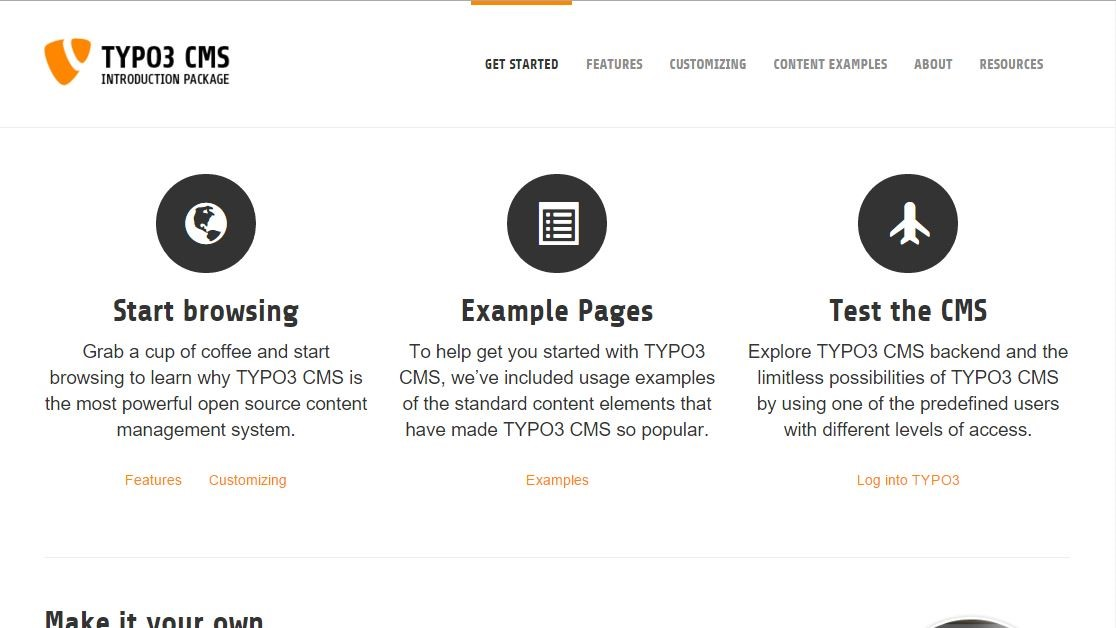
\includegraphics[scale=0.5]{abb/typo3frontend.jpg}
	\caption{Das Frontend gleicht einer normalen Website.}%
	\label{fig:typo3backend}
\end{figure}

\begin{figure}[ht]
	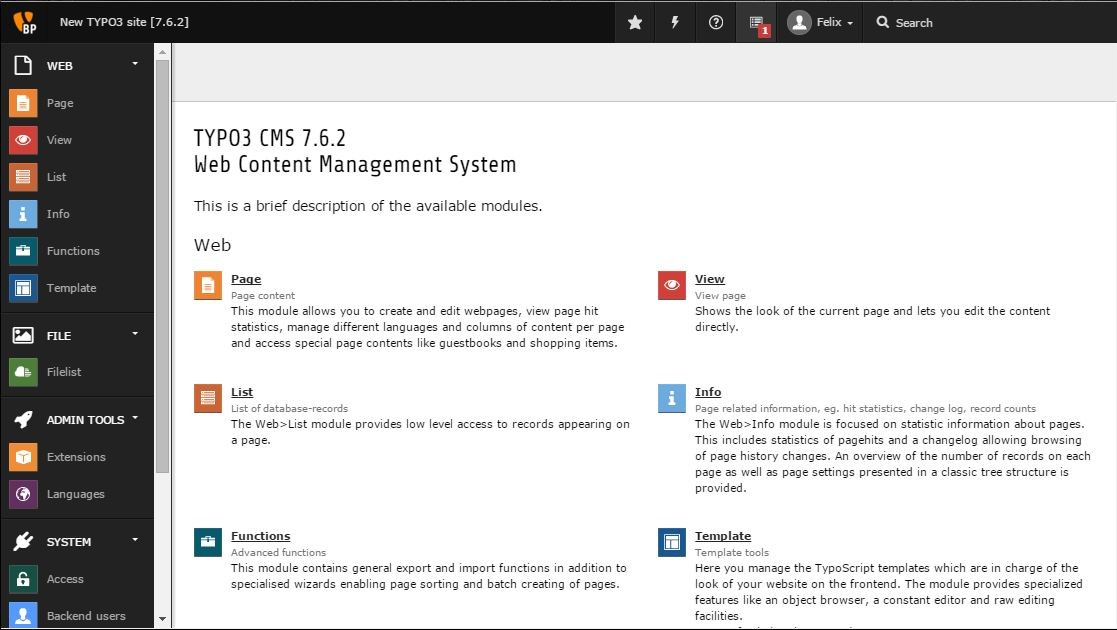
\includegraphics[scale=0.5]{abb/typo3backend.jpg}
	\caption{Das Typo3 Backend}%
	\label{fig:typo3backend}
\end{figure}

Das gr��te visuelle Merkmal der neuen Typo3 Version 7.6 LTS ist das neue, klarere Design des Backend von Typo3. So wird es f�r Anwender ohne Programmierkenntnisse einfacher sich zurechtzufinden und Inhalte zu erstellen. Dies geschieht haupts�chlich �ber einen integrierten WYSIWYG-Editor.

Dennoch enth�lt die Backend sehr viele Optionen, versteckte Kn�pfe und Eigenheiten, die einer Erkl�rung bed�rfen.

\section{Funktionalit�t und Architektur von Typo3}

Es handelt sich an dieser Stelle zwar um eine wissenschaftliche Arbeit und kein Handbuch, doch es ist ein wesentlicher Bestandteil dieser Arbeit, die Typo3 Umgebung zu verstehen um analysieren zu k�nnen, wie sie am geschicktesten auf die gesammelten Anforderungen anzupassen ist. Daher folgt nun eine komprimierte �bersicht �ber den Umgang und die Entwicklung von Typo3 Websites und den Workflow beim Erstellen dieser.

\subsection{Frontend Struktur}
Das Frontend ist die Seite, die ein normaler User zu sehen bekommt. Um diese als Entwickler manipulieren zu k�nnen muss man dessen Bestandteile kennen. Das Frontend ist grundlegend in vier Bereiche unterteilt.
\paragraph{Frontend Bereiche}
\begin{itemize}
	\item Header: Zeigt Inhalte ganz oben auf der Website, beispielsweise ein Logo.
	\item Men�: Beinhaltet das Hauptmen�.
	\item Content: Unterteilt sich in drei Teile, Links, Mitte und Rechts und stellt den eigentlichen Inhalt einer bestimmten Seite dar.
	\item Footer: Zeigt abschlie�ende Inhalte am Ende der Webseite
\end{itemize}

Wo genau diese Bereiche auftauchen und positioniert werden l�sst sich mittels eines Templates definieren, das mit Typoscript beschrieben wird. Im Backend finden sich genau diese Teile wieder und lassen sich dort mit Content bef�llen. Genaueres zu Templates und Typoscript wird weiter unten beschrieben.

\newpage
\subsection{Die Backend Module im �berblick}

Das Backend sieht seit dem Update deutlich einladender aus, die Bedienung gestaltet sich jedoch immer noch anspruchsvoller als bei vergleichbaren Konkurrenten. Deshalb folgt nun eine Erkl�rung der standardm��igen Men�punkte.\\
\begin{wrapfigure}{lph!}{0.25\textwidth}
	\begin{center}
		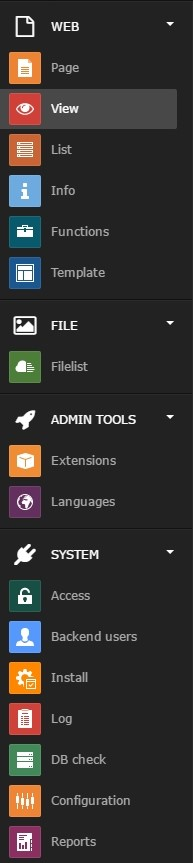
\includegraphics[width=0.25\textwidth]{abb/typo3menu.jpg}
	\end{center}
	\vspace{-10pt}
	\caption{Typo3 Backend Men�}
	\vspace{-240pt}
\end{wrapfigure}

\subsubsection{Page} 
Hier lassen sich die Einzelseiten der Webanwendung auf einem hohen Level erstellen und verwalten. Auch wenn noch keine Seite angelegt wurde, sieht man im Hierarchiebaum bereits einen Eintrag. Dieser stellt sozusagen die Wurzel aller zuk�nftigen Seiten dar, zeigt selbst jedoch keine Seite an. Haupts�chlich wird dieser Bereich genutzt um an den WYSIWYG-Editor zu kommen und in diesen neue Inhalte einzutragen oder Inhalte zu bearbeiten. 

\subsubsection{View} Hier ist es m�glich, das Frontend zu begutachten, ohne das Backend zu verlassen. Das kann n�tzlich sein, wenn schnell verschieden Aufl�sungen getestet werden sollen.
	
\subsubsection{List} In diesem Men�punkt findet sich eine �bersicht der Elemente, die dem Seitenbaum zugeordnet sind. Das k�nnen Webseiten oder auch Komponenten von Extensions sein. Oft wird diese Ansicht f�r erstellte Systemordner genutzt.

\subsubsection{Info} Hier lassen sich lediglich Informationen, wie zum Beispiel Erstellungsdatum oder welche Seiten in welcher Sprache verf�gbar sind, zu einzelnen Komponenten anzeigen.
	
\subsubsection{Functions} Dieser Bereich beherbergt einige n�tzliche Hilfsfunktionen, um schneller �nderungen, wie das Erstellen mehrerer Seiten gleichzeitig, durchzuf�hren. 
	
\subsubsection{Template} Hier werden alle Templates der Seite verwaltet. Dabei kann man das Template einer bestimmten Seite zuordnen oder ein Template auf die Wurzel der Seite setzen und somit global bereitstellen. Pro Template lassen sich hier vor Allem die Konstanen, das Setup und die Includes bearbeiten. Konstanten sind Dinge wie der Name der Webseite, Includes sind oft Stylesheets und im Setup wird via Typoscript die eigentliche Darstellungslogik des Templates programmiert.
	
\subsubsection{Filelist} Hier werden alle Dateien des sogenannten Filemount verwaltet. Alle f�r die Seite relevante Dateien k�nnen hier verwaltet werden. Meist handelt es sich um Dateien, die Redakteure in Eintr�ge integrieren. Auch schnelle �nderungen an CSS-Dateien lassen sich an dieser Stelle durch einen integrierten Texteditor vornehmen.
	
\subsubsection{Extensions} In diesem Bereich werden alle installierten Erweiterungen gelistet. Man hat dort die M�glichkeit diese zu aktivieren und deaktivieren. Zu bemerken ist, dass das nicht mit allen Erweiterungen m�glich ist, da einige Grundfunktionalit�ten von Typo3 auch als Erweiterungen gelistet sind und diese lassen sich nicht manipulieren. Dar�ber hinaus lassen sich hier neue Erweiterungen suchen und herunterladen. Der Extension Manager sucht dabei im Extension Repository von Typo3. Jede Extension hat hier einen einzigartigen Extension Key.
	
\subsubsection{Languages} Dieser Punkt hilft bei der Verwaltung von mehrsprachigen Seiten. Auch das Backend l�sst sich in mehreren Sprachen anzeigen.
	
\subsubsection{Access} Auf dieser Unterseite kann man sich einen �berblick �ber die Rechte verschiedener Usergruppen verschaffen. F�r jede Seite lassen sich die Rechte zum Ansehen, Editieren, L�schen und Erstellen von Unterseiten aller Gruppen �berpr�fen.
	
\subsubsection{Backend users} Hier lassen sich die Nutzer des Backend verwalten. Es lassen sich neue Backend User anlegen und auch spezifische Rechte dieser User konfigurieren. Typische Rollen sind Administrator/-in und Redakteur/-in. Es l�sst sich auch erkennen wer gerade im System eingeloggt ist.
	
\subsubsection{Install} Hier lassen sich durch das Install-Tool einige gravierende Einstellungen vornehmen, wie das Zur�cksetzen von Passw�rtern und �hnlichen Interaktionen mit der Datenbank. Au�erdem zeigt diese Unterseite die Konfigurationsdetails der Umgebung an. Dieser Bereich sollte nur Administratoren zug�nglich gemacht werden.
	
\subsubsection{Log} In diesem Bereich findet sich ein Protokoll �ber alle Nutzeraktionen und aufkommende Fehlermeldungen.
	
\subsubsection{DB check} Hier lassen sich Statistiken �ber die Eintr�ge der Datenbank anzeigen und Suchen in der Datenbank direkt durchs Backend durchf�hren.
	
\subsubsection{Configuration} In diesem Punkt findet sich lediglich eine recht un�bersichtliche Liste von Konfigurationsvariablen.
	
\subsubsection{Reports} Der Report liefert eine Liste von Nachrichten �ber den Lauf der Webseite und m�gliche Probleme.

\subsection{Typoscript}

Typoscript ist die Skriptsprache von Typo3. Es handelt sich dabei nicht um eine richtige Programmiersprache, was sich auch schon vom Namen her vermuten lassen k�nnte. Das zeigt sich auch in der Art und Weise wie Typoscript von Typo3 verarbeitet wird, n�mlich als sehr langes PHP Array und einem internen Parser. Typoscript ist mehr daf�r ausgelegt dem Ersteller der Webseite eine M�glichkeit zu geben, zu bestimmen, wie Typo3 mit bestimmten Objekten, wie zum Beispiel Bildern, Men�s oder Templates, umgehen soll. Es ist so also haupts�chlich f�r die spezifische Ausgabe von Content zust�ndig.
In Typoscript wird immer mit Objekten gearbeitet, denen man bestimmte Eigenschaften zusprechen kann.

Eine Typoscript Datei, die in jedem Template enthalten ist, ist die setup.ts. Aus der Setup Datei des Standard-Templates ist nun ein kleiner Schnipsel zu sehen.

\begin{verbatim}
page = PAGE
page{
 includeCSS.style = fileadmin/Template_WegE/bootstrap/css/style.css

 10 = FLUIDTEMPLATE
 10{
  file = fileadmin/Template_WegE/index.html
  layoutRootPath = fileadmin/Template_WegE/layouts/
  partialRootPath = fileadmin/Template_WegE/partials/

  variables{
	siteName = TEXT
	siteName.value = WegE Fallstudie

	content < styles.content.get
  }
 }
}
\end{verbatim}

Zu Beginn wird eine Variable mit dem Namen page gesetzt, welche die ganze Seite pr�sentiert. Das gro�geschriebene PAGE ist ein Objekt und die vorgegebene Weise, die komplette Seite anzusprechen. Diese bekommt in Zeile 3 ein neues Stylesheet zugewiesen, das dann automatisch eingebunden wird. Danach wird eine Variable zum Fluidtemplate. Die Zahl 10 pr�sentiert dabei einen Platz im PAGE Array, das danach aus Typoscript generiert wird. Hier ist die Reihenfolge oft wichtig. Es ist �blich Anweisungen mit in Zehner-schritten zu nummerieren, sodass man sp�ter eventuell vergessene Anweisungen noch zwischen zwei Zahlen einf�gen kann. F�r das Fluidtemplate werden nun die Pfade zu den Layouts und Partials definiert. Layouts und Partials sind Einzelteile eines Templates. Genaueres dazu im Verlauf dieses Kapitels.
Darunter wird noch mittels Typoscript der Name der Seite definiert, welcher sp�ter an vielen Stellen verwendet werden kann.

\subsection{Erweiterungen/Extensions}

Ein gro�er Vorteil und Grund f�r die Wahl von Typo3 als CMS sind die Erweiterungen oder Extensions. Mit diesen Extensions l�sst sich das CMS mit wenig Aufwand um etliche Features erweitern. Inzwischen existieren tausende von Erweiterungen f�r Typo3. \textquotedblleft Extension \textquotedblright ist dabei ein �berbegriff f�r verschiedene Arten von Erg�nzungen\cite{typo3CoreApi}\cite{Ebner2010}:

\begin{itemize}
	\item \textbf{Plugins} sind Erweiterungen des Frontend, wie zum Beispiel ein G�stebuch. Im den Extension Kategorien werden Plugins unter Frontend oder Frontend-Plug-in gelistet. Frontend Plug-in Extensions erzeugen dabei eine eigene Ausgabe, w�hrend das Gegenst�ck diese Ausgabe lediglich beeinflusst.
	\item \textbf{Module} sind Backend Erweiterungen und f�gen diesem meist auch einen neuen Men�punkt hinzu. In den Extension Kategorien werden Module unter Backend oder Backend-Modul gelistet. Backend-Module sind dabei diejenigen mit eigenem Men�punkt.
	\item \textbf{Services} sind libraries, die Vorteile durch die Nutzung einer API bieten. Sie tragen den selben Namen unter den Extension Kategorien.
	\item \textbf{Distributionen} sind vollst�ndige CMS Installationen, als Paket vorgefertigt. 
	\item Die restlichen Extension Kategorien hei�en Documentation, Templates, Examples und Miscellaneous. Diese enthalten genau das was der Name verspricht. Miscellaneous dient als Auffangbecken f�r alle Extensions, die sich nicht zuordnen lassen.
\end{itemize}

Dar�ber hinaus gibt es Systemextensions, welche zum Kern von Typo3 geh�ren und nicht manipuliert werden k�nnen.

Bei der Anzahl von tausenden Extensions muss allerdings dazugesagt werden, dass ein gro�er Teil dieser veraltet ist, nicht mehr gepflegt wird oder gar �berhaupt nicht auf der neuen Version lauff�hig gemacht werden kann. Das liegt auch daran, dass viele der Extensions von freien Programmierern in ihrer Freizeit entwickelt werden. So gilt es etwas vorsichtig bei der Auswahl passender Extensions zu sein.
Zu finden sind diese Extensions auf der offiziellen Seite im Extension Repository\footnote{typo3.org/extensions/repository}. Jede Extension findet sich hier unter einem einmaligen Extension Key wieder. Wichtig ist es auf die Kompatibilit�t zur eigenen Typo3 Installation zu achten, die dort angezeigt wird. Auch findet sich hier meist eine Dokumentation zur Einrichtung und weiteren Infos zur jeweiligen Erweiterung. Extensions selbst k�nnen Abh�ngigkeiten zu anderen Extensions haben, die vorher installiert sein m�ssen um lauff�hig gemacht zu werden. Selten gibt es auch Konflikte zwischen zwei Extensions, was zu Fehlern f�hren kann. Solche sollte man also nicht gleichzeitig auf einem System installieren.
Die Erweiterungen der eigenen Typo3 Anwendung lassen sich durch den Men�punkt \emph{Erweiterungen} im Backend verwalten.

\subsection{Templates erstellen}

Beim Erstellen einer Typo3 Website bekommt der Entwickler f�r gew�hnlich ein Frontend Design der Seite geliefert und hat dann die Aufgabe dieses Design in Typo3 zu integrieren. Das geschieht durch das Schreiben von Typoskript, das Installieren von Extensions, der Anpassung des Backend und die Entwicklung von Templates. Der Begriff Template ist bei Typo3 mehrfach belegt, deshalb vorerst eine Unterscheidung:

\begin{itemize}
	\item HTML-Template: Die statische HTML-Vorlage, welche meist ein Designer liefert.
	\item TypoScript-Template: Alle Typoscript-Anweisungen, die Ausgabe von Men�s und �hnlichem steuern liegen im Typoscript-Template.
	\item Fluidtemplate: Mit Typo3 lassen sich im HTML-Code Fluid-Funktionen  verwenden. Diese erlauben Variablen und Bedingungen innerhalb des HTML. Au�erdem erlaubt es das Aufteilen des HTML-Codes in Partials.
\end{itemize}

Ein Typo3 Fluidtemplate besteht also aus einem Layout, das Dinge wie head und header enthalten kann, einem Template, das den Inhalt repr�sentiert und Partials, die mehrmals auf einer Seite vorkommen k�nnen.

\begin{figure}
\centering
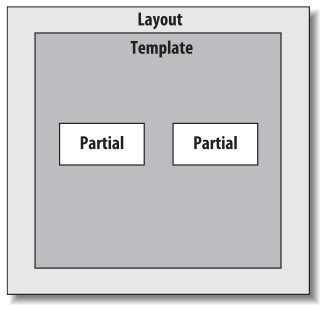
\includegraphics[width=0.5\linewidth]{abb/typo3_template_overview.png}
\caption[Typo3 Template Teile]{Typo3 Template Komponenten}
\label{fig:typo3_template_overview}
\end{figure}

Im Folgenden geht es vor Allem um das Fluidtemplate, welches aus dem HTML-Template erzeugt wird. F�r das Fluidtemplate ist es heutzutage �blich eine Template-Extension zu erstellen. Das bedeutet, dass das Template in einzelnen Dateien auffindbar ist, statt in der Datenbank, was die Versionierung und Weitergabe eines Templates erheblich vereinfacht. Da die Teamarbeit durch Dienste wie Git �u�erst popul�r geworden ist, wird diese Methode der Template-Entwicklung bevorzugt.

Zu Beginn einer neuen Template-Extension hilft eine Typo3 Extension weiter. Diese findet sich unter dem Namen \textit{extension\_builder}. Dieser Builder erzeugt im Backend einen neuen Men�punkt unter dem sich im Unterpunkt Domain Modeling eine neue Template-Extension erstellen l�sst. Diese taucht dann auch in der Extension-Liste auf.

F�r die Arbeit mit den Dateien des erstellten Templates wird ein externer Editor ben�tigt. Im besten Fall sollte dieser auch mit Typoscript umgehen k�nnen, was die Wahl deutlich einschr�nkt. Zwei gute Optionen sind hier die IDEs UltraEdit und Webstorm. 

Da der Fokus dieser Arbeit mehr auf der Umsetzung funktionaler Anforderungen liegt, wird an dieser Stelle nicht weiter auf die M�glichkeiten zum Designen von Typo3 Webseiten eingegangen. F�r die beispielhafte Umsetzung der Anforderungen wird ein einfaches Bootstrap Ger�st verwendet, dessen Implementation im Anhang zu finden ist.

\subsection{Beispielinstallation}

In diesem Unterpunkt wird der tats�chliche Installationsprozess der Testumgebung, inklusive einem Blick auf den Code, dokumentiert. Da sich diese Installationsanleitung sehr praktisch gestaltet, sollten die Versionen der genutzten Software beachtet werden, da hier schnell �nderungen auftreten k�nnen. Die Testumgebung l�uft mit Typo3 7.6 LTS und Wamp 3.0.0 mit PHP 5.6. Wichtig hierbei ist vor Allem die Typo3 Version. Es wird mit Bootstrap Version 3 gearbeitet.

\paragraph{Typo 3 Installationsschritte}
\begin{enumerate}
	
	\item Typo3 7.6 LTS herunterladen.
	\item Wamp oder vergleichbares Programm herunterladen und installieren.
	\item Den Typo3 Ordner in den \texttt{www}-Ordner von Wamp (htdocs bei XAMPP) verschieben
	\item Nach dem Starten von Wamp zu \texttt{localhost/\textit{typo3Ordner}} navigieren.
	\item Es erscheint ein Installationsguide und wahrscheinlich eine Reihe von Fehlern, die zu beheben sind
	\item Die \texttt{php.ini} �ffnen
	\subitem Die Variable \texttt{memory\_limit} erh�hen auf 64 oder h�her
	\subitem Die Variable \texttt{upload\_max\_filesize} auf mindestens 10MB erh�hen
	\subitem Die Variable \texttt{max\_execution\_time} auf 240 setzen
	\item Die OpenSSL Extension muss als Systemvariable gesetzt werden. Unter Systemvariablen die Variable mit dem Namen \texttt{OPENSSL\_CONF} und dem Wert des Pfades zur openssl.cnf angeben. Danach eventuell Computer neu starten.
	\item Die PHP Extension Fileinfo geht nicht. In der php.ini das Semikolon vor \texttt{extension=php\_fileinfo.dll} entfernen.
	\item Windows Apache Thread Stack Size Fehler. Dieser kann in der httpd.conf Datei angepasst werden. Hier folgenden Codeschnipsel ans Ende der Datei kopieren:\\ \texttt{<IfModule mpm\_winnt\_module> ThreadStackSize 8388608 </IfModule>}
	\item Alle Dienste von Wamp neu starten und zum Installationstool von Typo3 zur�ckkehren. Im n�chsten Schritt wird eine Datenbank ben�tigt. Will man diese selbst anlegen hilft das Tool phpmyadmin unter localhost/phpmyadmin. Hier l�sst sich mit einem Klick eine leere Datenbank anlegen.
	\item Typo3 verlangt beim Anlegen der Datenbank auch den Port. Dieser l�sst sich in der Konsole mit dem Befehl netstat -a -o auslesen. Hierzu vergleicht man die angezeigte PID mit dem Wamp Prozess im Taskmanager. F�r gew�hnlich ist der Port eine Zahl um die 3000.
	\item Nun l�sst sich das Backend, durch das Anh�ngen von /typo3 in der Adresszeile, aufrufen.
	
\end{enumerate}

\paragraph{Template-Erstellung Schritte} 

Der Vorteil eines CMS ist die Erstellung von dynamischem Content. Um das zu bewerkstelligen braucht es ein Template zum Anzeigen dieser Inhalte. F�r die Testumgebung wurde ein rudiment�res Template basierend auf dem Bootstrap Framework installiert. Das Bootstrap Framework sorgt ohne viel Arbeit f�r ein besseres Aussehen der Webseite und Responsivit�t, d.h. eine automatische Anpassung an alle Bildschirmgr��en.


\begin{enumerate}
	
	\item Bootstrap 3 herunterladen.
	\item Bootstrap Starter Template herunterladen durch das Kopieren des Quellcodes (F12). Diese vorerst als \texttt{index.html} abspeichern.
	\item In der \texttt{index.html} alle href-Links an die neue Umgebung anpassen. Der vollst�ndige Code findet sich im Anhang.
	\item Einen neuen Ordner im Verzeichnis fileadmin anlegen. Dieser h�lt das Template.
	\item Hier die \texttt{index.html} und den bootstrap Ordner ablegen. Dazu drei neue Ordner anlegen mit den Namen \texttt{layouts}, \texttt{partials} und \texttt{ts}.
	\item Im Backend unter dem Men�punkt Template muss das Bootstrap Template im Root der Webseite angelegt werden. Sollte dieser nicht existieren, kann dieser unter \texttt{Page} angelegt werden.
	\begin{figure}
		\centering
		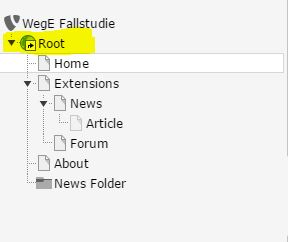
\includegraphics[width=0.3\linewidth]{abb/roottemplate.jpg}
		\caption{Aufbau des Website-Baumes}
		\label{fig:roottemplate}
	\end{figure}
	\item Im Root-Template unter \texttt{Includes} m�ssen zwei Dinge eingef�gt werden, \texttt{css\_styled\_content} und \texttt{fluid\_styled\_content}. Die Reihenfolge ist dabei wichtig. Sollte \texttt{fluid\_styled\_content} nicht existieren, muss dieses als Extension installiert werden.
	\item Unter \texttt{General} werden nun zwei externe Typoscript Dateien f�r die Konstanten und das Setup verlinkt. So erh�lt man mehr Flexibilit�t bei der Arbeit mit Versionierungen und Teamarbeit.
	\subitem Unter \texttt{Constants} wird Folgendes geschrieben: \texttt{<INCLUDE\_TYPOSCRIPT: source=" FILE:fileadmin/\textit{Template\_WegE}/ts/constants.ts">}
	\subitem Unter \texttt{Setup}: \\
	\texttt{<INCLUDE\_TYPOSCRIPT: source= " FILE:fileadmin/\textit{Template\_WegE}/ts/setup.ts">}
	\subitem Die zwei verlinkten Dateien m�ssen nun auch im ts-Ordner erstellt werden.
	\item Die setup.ts ben�tigt nun einiges an Code, der aus der index.html �bertragen wird. Diese enth�lt dann nur noch den Code zwischen den body-tags. Die fertige Datei ist im Anhang zu finden. 
	\item Die Teile aus der index.html, die nun wegfallen, werden in der setup.ts angelegt. Daf�r ist ein PAGE Objekt n�tig, welches alle referenzierten Dateien, wie bootstrap.css, einbindet. Die komplette Datei ist im Anhang zu finden. Die Inhalte, die das Template der Testumgebung dynamisch erstellt werden sollen beschr�nken sich auf das Men� und den Seitentitel. Nachdem diese Datei angelegt ist, wird das Men� automatisch mit den erstellten Seiten aus dem Typo3 Backend gef�llt.
	
\end{enumerate} 

Nach dem Anlegen eines rudiment�ren, aber voll funktionsf�higem Template, kann mit dem Erstellen von Content, beziehungsweise dem Installieren und Testen von Extensions, begonnen werden.

\chapter{Anpassung eines Typo3 Systems an die gesammelten Requirements}
\label{kap-typo3praxisteil}

Nach dem Erstellen einer simplen Typo3 Umgebung ist das Ziel dieses Teils die Untersuchung verschiedener Extensions, die zur Umsetzung der WegE Requirements genutzt werden k�nnen. Um die besten Extensions ausw�hlen zu k�nnen, werden einige sinnvolle Kriterien ben�tigt. Nur wenige dieser Kriterien lassen sich generell auf alle Extensions anbringen. Wie auch bei der Wahl des CMS gibt es nicht die eine beste L�sung, sondern viele Optionen, die eigens gegeneinander abgew�gt werden m�ssen. Nichtsdestotrotz sollte jede ernst zu nehmende Extension einige Punkte erf�llen.

\paragraph{Eigenschaften einer professionellen Extension}
\begin{itemize}
	\item \textbf{Einhalten der Typo3 Coding Guidelines}: Diese Guidelines decken die wichtigsten Aspekte einer guten Extension, wie Sicherheit, Erweiterbarkeit, Stabilit�t und Zukunftssicherheit, ab. https://docs.typo3.org/typo3cms/CodingGuidelinesReference/Index.html
	\item \textbf{Kompatibilit�t mit eigenem Typo3 System}: Nat�rlich soll die Extension f�r die jeweilige Version verf�gbar sein und nicht im Konflikt mit anderen Extensions stehen. Au�erdem sollte die Lizenz der Extension beachtet werden.
	\item \textbf{Extension Manual verf�gbar} Eine offizielle Anleitung kann direkt auf der Downloadseite der Extension auf Typo3 verlinkt werden und ist unerl�sslich f�r den richtigen Umgang mit einer Extension und sollte nicht fehlen.
\end{itemize}

Die erste Anlaufstelle zur �berpr�fung dieser Eigenschaften ist die Downloadseite der Extension auf typo3.org. Diese bietet eine �bersicht �ber Version, Update, Alter, Kategorie, Autor und Downloadzahlen einer Extension. Die Anzahl der Downloads ist meistens ein guter Indikator f�r eine professionelle Extension, jedoch nicht immer. Deshalb sollte dieser mit Vorsicht genossen werden.

\begin{figure}
	\centering
	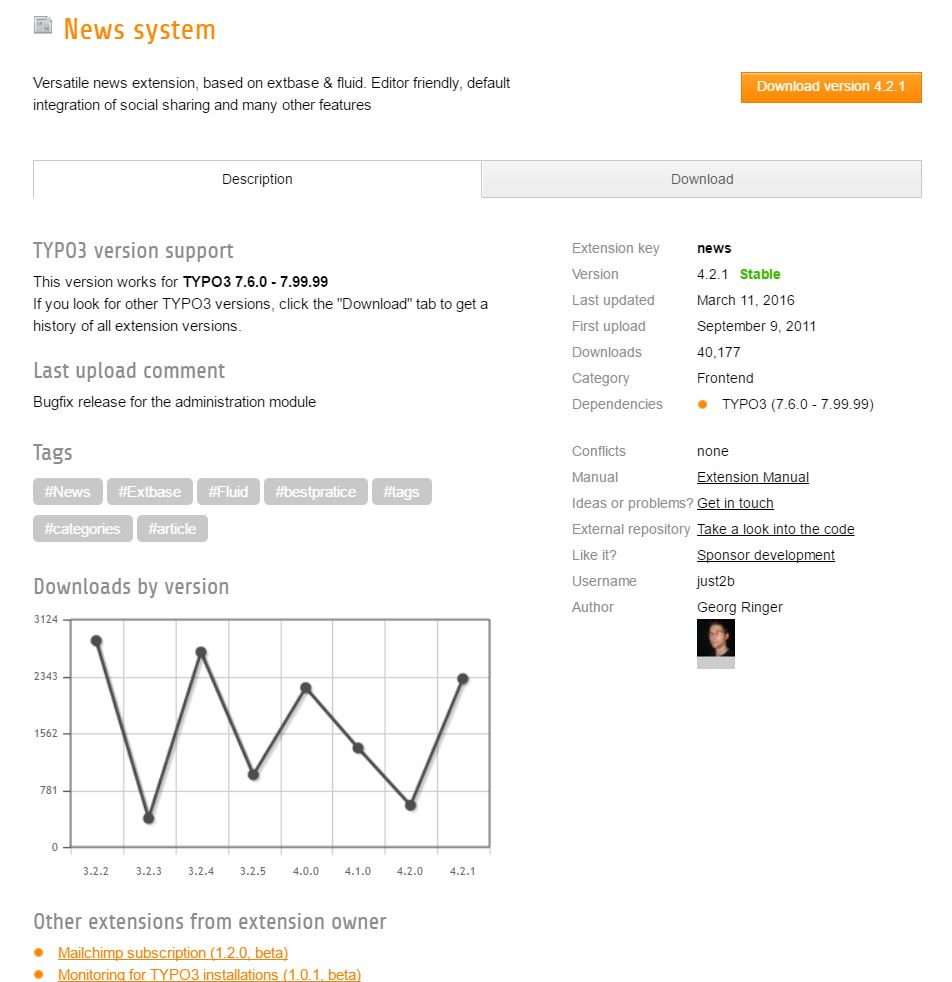
\includegraphics[width=0.75\linewidth]{abb/extensionseite.jpg}
	\caption[Extension �bersicht]{�bersicht einer Extension auf der Downloadseite}
	\label{fig:forumextension}
\end{figure}

Neben den oben genannten Kriterien gibt es noch ein hilfreiches Projekt namens Extension Comparison project\footnote{https://wiki.typo3.org/Extension\_Comparison} auf der Typo3 Wiki Webseite, die ein gro�e Anzahl von Extensions gleicher Art jeweils vergleicht und so die Wahl erleichtert.

F�r das WegE Projekt kommen prinzipiell nur professionelle Extensions in Frage. Besonders wichtig sind die Zukunftssicherheit und Stabilit�t. Dar�ber hinaus spielt der Aufwand eine wichtige Rolle. Lizenzkosten sollen m�glichst vermieden werden.  

\section{Rechtemanagement und Authentikation}
Die Erstellung und das Management der Usergruppen, die f�r das WegE Projekt geplant sind, k�nnten sich als eine der schwierigsten Aufgaben entpuppen. Zum einen gibt es eine Menge Redakteure, f�r viele verschiedene Sektionen der Webseite. Dann soll es die M�glichkeit geben sich mittels Kennnummer der Universit�t einzuloggen und zum Schluss soll jeder interessierte User sich einen Account anlegen k�nnen, um zum Beispiel im Forum mitzuwirken. Daraus resultiert ein kompliziertes Rechtemanagement.

Wichtig hierbei die Unterscheidung von Backend Usern und Frontend Usern. Das Erstellen von Backend Usern l�sst sich bequem �ber das Backend von Typo3 erledigen. Ein Administrator legt daf�r einfach einen neuen Nutzer an und bestimmt die jeweiligen Rechte dieses Nutzers. Das werden zumeist Redakteure sein und da sich die Zahl dieser in Grenzen halten sollte, ist es m�glich diese alle manuell anzulegen.

\subsection{M�glichkeiten}

Braucht eine Webseite nur Administratoren und einige Redakteure, also nur Backend User, so l�sst sich das nur mit Typo3 allein bewerkstelligen. Daf�r legt ein Administrator per Hand im Backend manuell neue Zug�nge an. Das funktioniert nicht mit Frontend Usern.
Die momentan vorherrschende Methode zur Verwaltung von Frontend Usern ist die Extension sr\_feuser\_registration. Sie befindet sich in den meist heruntergeladenen Extensions, wurde bereits 2005 das erste mal ver�ffentlicht und wird in Version 4.0 angeboten. 


\subsection{Implementation}

Die Implementation dieser Extension verl�uft, in Ber�cksichtigung der Gr��e des Vorhabens, sehr schnell ab.

\begin{figure}
	\centering
	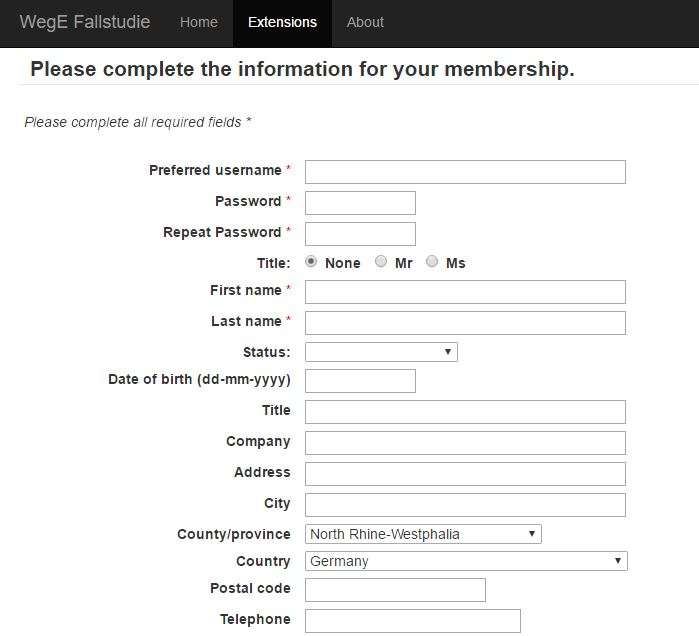
\includegraphics[width=0.75\linewidth]{abb/fe_user.jpg}
	\caption[sr\_feuser\_register Extension]{Das erzeugte Registrierungsformular}
	\label{fig:feusersextension}
\end{figure}

\subsection{Evaluation}

Die Arbeit mit der sr\_feuser\_registration Extension stellte sich als sehr angenehm heraus. Das mag mitunter daran liegen, dass sie sich seit �ber 10 Jahren in Entwicklung befindet und in einem sehr ausgereiften Stadium befindet. Die Extension bietet so gut wie jede erdenkliche Funktion rund um das Thema Frontend User als Men�punkt im Backend, sodass man schnell und ohne Anleitung ein funktionierendes Registrierungsformular aufsetzen kann. Es nutzt die bereits vorhandenen Funktionen von Typo3, womit es sich leicht definieren l�sst, welche Seiten nur f�r registrierte User gedacht sind. Sind Frontend User auf einer Typo3 Seite n�tig ist diese Extension eine optimale L�sung. Dar�ber hinaus gibt es viele Extensions, welche die Funktion von sr\_feuser\_registration erweitern.

\section{Blog und News}
Die Anzeige von News oder einem fortlaufenden Blog findet auf immer mehr Webseiten Relevanz. So ist es wenig verwunderlich, dass die bekannteste News-Extension von Typo3 auch eine der meistverwendeten Extensions �berhaupt ist. Die popul�rste Wahl scheint dabei die Extension mit dem Namen \texttt{news} zu sein.

\subsection{Alternativen}
Eine weitere Extension, die f�r die Anzeige eines Blogs geeignet ist, hei�t typo3\_blog. Die Extension steht der vorgestellten news Extension in Nichts nach, jedoch bietet die news Extension zwei Dinge in einem, news und Blog Funktionalit�t und deckt somit zwei m�gliche Anforderungen der WegE Plattform ab. Somit minimiert die Wahl der news Extension theoretisch Installationsaufwand.

\subsection{Implementation}
Zu Beginn eine kleine Warnung: Eine Extension mit dem Namen \texttt{tt\_news} ist nicht mehr lauff�hig und sollte nicht mit der Extension \texttt{news} verwechselt werden.\\
Nach dem Installieren der Extension findet sich im Men� des Typo3 Backend ein neuer Unterpunkt. Hier lassen sich neue News anlegen und verwalten. Vorerst m�ssen jedoch einige Seiten zur Anzeige der News angelegt werden. Im Page Men� erstellt man dazu eine Seite zum Anzeigen der �bersicht aller News. Hier werden kleine Vorschauen der News in einer Liste angezeigt. Dazu muss des Weiteren eine Unterseite zur News �bersichtsseite angelegt werden. Hier wird eine volle News angezeigt, sofern der User auf der �bersichtsseite auf den Auszug einer News klickt. Als letztes wird noch ein Ordner ben�tigt, in dem alle News gespeichert werden. Dieser wird im Webseitenbaum angelegt.\\
Beim Erstellen von Content auf der News �bersichtsseite und einem Klick auf Normal->Content, findet sich oben im Men� der Reiter Plugins. Hier taucht auch das News System auf. Dieses muss noch ein zweites Mal auf der Detailseite hinzugef�gt werden. \\
Um diese Funktionalit�t der Detailseite zu bewerkstelligen m�ssen nach dem Erstellen dieser Seiten im Plugin einige Angaben gemacht werden. Beim Editieren des Plugins auf der News �bersichtsseite unter dem Reiter Plugin muss die List view ausgew�hlt sein. Diese erzeugt die gew�nschte �bersicht aller News. Im Unterreiter Additional wird angegeben welche Seite f�r die Detailansicht verantwortlich sein soll. Im Plugin der Detailseite ist f�r die Detailansicht Detail view zu w�hlen und eine Referenz auf die �bersichtsseite zu setzen.\\
Unter dem News Men�punkt lassen sich nun neue Artikel mit Tags, Bildern, Kategorien, Autor etc. erstellen, die bereits, wie gewollt, angezeigt werden.\\
Die Extension kommt mit einem eigenen Design daher, was f�r eine seri�se Anwendung nat�rlich angepasst werden m�sste. F�r diese Testumgebung bleibt es jedoch beim Standard-Design.
\begin{figure}
\centering
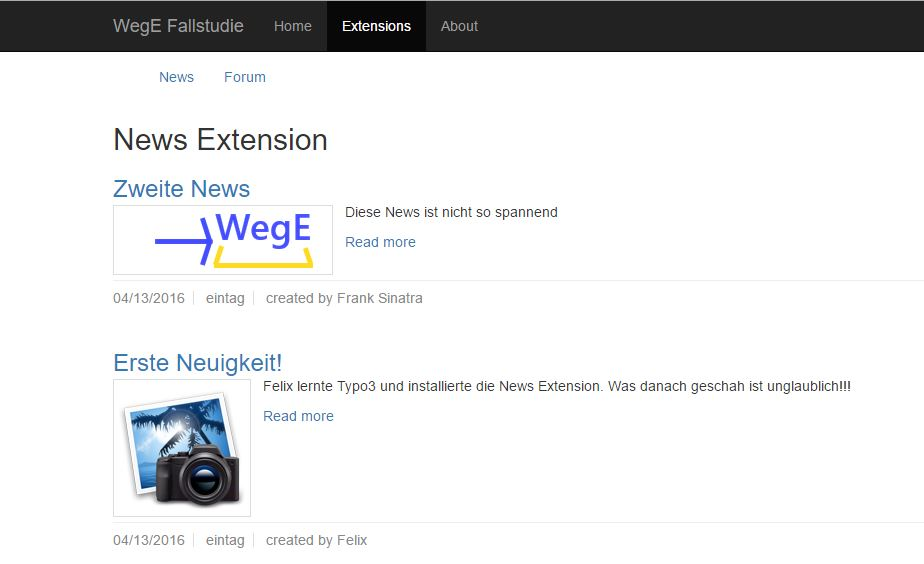
\includegraphics[width=0.75\linewidth]{abb/newsextension.jpg}
\caption[News Extension]{Das Ergebnis der news Extension}
\label{fig:newsextension}
\end{figure}


\subsection{Evaluation}
Die \texttt{news} Extension bietet alle Funktionalit�ten, die man f�r die Anzeige von News jemals brauchen wird. Die Implementation geht schnell, wenn auch nicht unbedingt beim ersten Mal. Alles in Allem ist diese Extension eine exzellente Wahl.

\section{Forum}

Die Anforderung an ein Forum ist mit Sicherheit eines der aufw�ndigsten Teile dieses Projekts. Das bedeutet auch, dass eine hochwertige Extension hier eine gro�e Zeitersparnis bedeuten kann. Ein Forum soll bestimmten Nutzern erlauben neue Themen anzulegen. Diese Themen werden in Listen angeordnet und das Klicken eines Themas f�hrt zu einer Unterseite, in der User dieses Thema diskutieren k�nnen. Der Content besteht dabei nicht nur aus Text, sondern auch aus Bildern und eventuell aus Dateianh�ngen. Dazu soll es Funktionalit�t geben, all diesen Content editieren und l�schen zu k�nnen und dabei diese Funktionalit�t sinnvoll nur bestimmten Nutzern zu geben. So soll zum Beispiel nur der Ersteller ein Thema wieder l�schen k�nnen. Erreicht ein Forum eine bestimmte Gr��e ist es w�nschenswert eine weitere Usergruppe definieren zu k�nnen, die ein Forum moderieren und somit die Rechte besitzen jegliche Anpassungen vorzunehmen. 

\subsection{M�glichkeiten}

Es gibt eigentlich nur eine Extension, die f�r Typo3 7.6 in Frage kommt und die hei�t typo3\_forum. Sollte diese aus irgendwelchen Gr�nden als M�glichkeit ausscheiden kann man auf ein externes Forum Plugin zur�ckgreifen, das auf einer niedrigeren Ebene integriert wird. Ein etabliertes Beispiel hei�t phpBB und bietet genau diese Funktionalit�t. Tats�chlich bietet phpBB mehr Anpassungsm�glichkeiten als die typo3\_forum Extension, ist aber auch mit etwas mehr Arbeit verbunden, da man aus der Typo3 Umgebung ausbricht.

\subsection{Implementation}

Die Implementation der grundlegensten Forum-Funktionalit�t f�llt moderat aus. Nach der Installation wird ein Sysfolder ben�tigt und ein spezieller Forum-Record angelegt. In diesem lassen sich die Rechte f�r jegliche Funktionen genau anpassen. Beispielsweise welche Usergruppen in der Lage sind Antworten zu posten. Au�erdem wird das Root Template mit der Extension erweitert. Zuletzt kommt man nicht drum herum etwas Typoscript zu schreiben. Es handelt sich hierbei jedoch nur um einen kleinen Schnipsel, der die Orte zur Anzeige des Forums und des Speichers �ber die PID definieren. Zus�tzlich ist zu beachten, dass MySQL nicht im strict mode sein darf. Das l�sst sich in der my.ini abschalten.

\begin{figure}
	\centering
	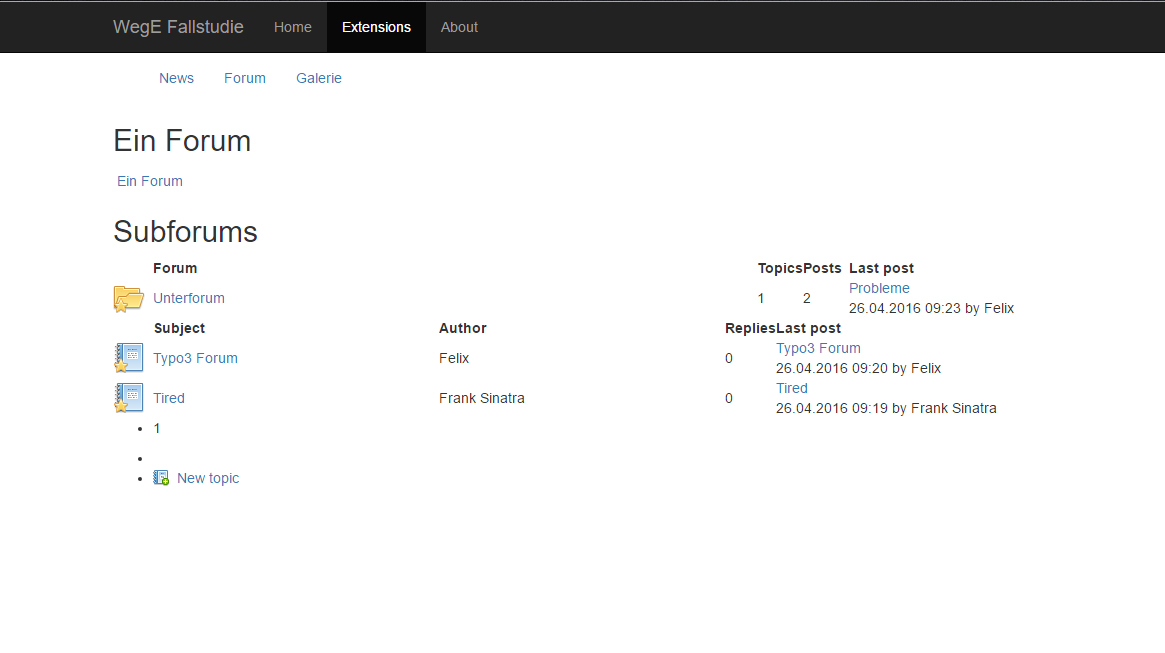
\includegraphics[width=0.75\linewidth]{abb/forumextension.png}
	\caption[Forum Extension]{Das Ergebnis der typo3\_forum Extension}
	\label{fig:forumextension}
\end{figure}

\subsection{Evaluation}

Grunds�tzlich bietet dieses Forum alle Funktionen, die f�r ein vern�nftiges WegE Forum n�tig sind. Leider existieren zu diesem Zeitpunkt noch einige schwer nachvollziehbare Bugs. Ein Beispiel hierf�r sind die Buttons zum Erstellen eines neuen Forumeintrages, die nicht immer angezeigt werden, wenn sie es sollten. Diese lassen sich durch individuelle Anpassungen soweit vermeiden, das bedeutet wiederum merh Aufwand. Da diese Extension jedoch noch sehr neu ist und von einem professionellen Team betreut wird, ist es gut m�glich, dass sich dieser Fakt bereits in wenigen Monaten �ndert.

\section{Anbindung an bestehende Systeme durch Datenimport}

\subsection{M�glichkeiten}

external\_import

\subsection{Implementation}

\subsection{Evaluation}

\section{Eigene Contentelemente}

�blicherweise bekommt ein Redakteur beim Erstellen eine Seite zu Gesicht, die sich grob in bestimmte Positionen auf der Seite gliedert. Mit einem Klick auf ein Plus in einem der Positionen taucht eine Auswahl von verschiedenen Content Elementen auf. So l�sst sich beispielsweise eine Tabelle oder ein ganzer WYSIWYG Bereich hinzuf�gen. Sp�testens wenn man Elemente mit komplizierterem Design auf einer Webseite platzieren will, werden st�rkere Tools ben�tigt. Durch das Hinzuf�gen eigener Content Elemente lie�e sich der Output viel besser steuern und vorab so designen, dass der Redakteur sich darum keine Gedanken machen muss. Redakteure k�nnten weniger falsch machen und w�rden sich gleichzeitig besser zurechtfinden. Das Beispiel im WegE Projekt, das Gebrauch von dieser Funktionalit�t machen w�rde, ist eine Promobox, die am Rand der Webseite auftauchen soll und auf verschiedenes aufmerksam machen soll.

\begin{figure}[h]
	\centering
	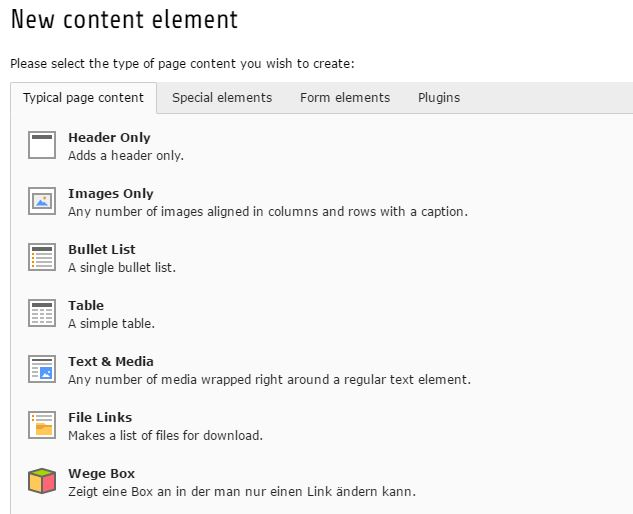
\includegraphics[width=0.75\linewidth]{abb/wegebox.jpg}
	\caption[Neues Content Element]{Das neue Content Element ist direkt in der Liste der Standard Elemente ausw�hlbar}
	\label{fig:forumextension}
\end{figure}

\subsection{M�glichkeiten}

Prinzipiell ist es m�glich alle angelegten Content Elemente von anderen Seiten zu kopieren und nochmals einzuf�gen. F�r das Beispiel einer WegE Promobox ist diese L�sung jedoch aus mehreren Gr�nden nicht optimal. Zuerst m�sste ein Redakteur bereits eine ansprechende Box nur mit Hilfe des WYSIWIG Editors angelegt haben. Dann m�sste jeder, der diese Box nutzen will, wissen in welchen Seiten sie zu finden ist um sie zu kopieren.
Bessere Alternativen bietet eine passende Extension namens Dynamic Content Elements (dce)\footnote{https://docs.typo3.org/typo3cms/extensions/dce/}. Sie erlaubt das Anlegen neuer Content Elemente und das Manipulieren dieser mittels Fluidtemplate. Die Extension wird bereits seit 2012 angeboten und ist �ber 25,000 Downloads sehr beliebt. Sie hat keinerlei Anforderungen oder Konflikte mit anderen Extensions.

\subsection{Implementation}

Die Implementation eines kleinen Beispiels ist sehr einfach. Nach dem Download der Extension lassen sich im neuen Men�punkt DCE eigene Content Elemente erstellen. Hierf�r lassen sich so viele verschiedene Input Felder wie n�tig anlegen. Im Falle des Beipiels nur eins. Das Input Feld bekommt dann einen Variablennamen, in diesem Fall \texttt{wgppb}. Dieser Variablenname findet im n�chsten Schritt Verwendung. Direkt im Backend l�sst sich das Fluitemplate f�r die Anzeige des Content Elements schreiben. Alle Input Felder lassen sich nun hier einarbeiten. Im Beispiel passiert das mit \\texttt{{field.wgppb\}}.

\paragraph{Fluidtemplate der Promobox}
\begin{verbatim}
	{namespace dce=ArminVieweg\Dce\ViewHelpers}
	<f:layout name="Default" />
	
	<f:section name="main">
	<div style="max-width: 220px; background-color: #cecece;
	   border-radius: 10px; padding: 10px;">
	 <h2>Promobox</h2>
	 <f:image src="uploads/pics/wege_logo.png" alt=""/>
	 <p>Diese Promobox ist mit DCE erstellt worden!</p>
	 <p>Der Redakeuter darf nur bestimmen wo der folgende Link hinf�hrt.</p>
	 <a href="{field.wgppb}">Klick mich</a>
	</div>
	</f:section>
\end{verbatim}

Dar�ber hinaus l�sst sich das Aussehen des Content Elements in der Auswahl f�r Redakteure ver�ndern. Beim Einbinden der WegE Promobox taucht lediglich ein Feld auf und verlangt nach einem Link. Alles andere wurde vom Fluidtemplate �bernommen.

\begin{figure}[h]
	\centering
	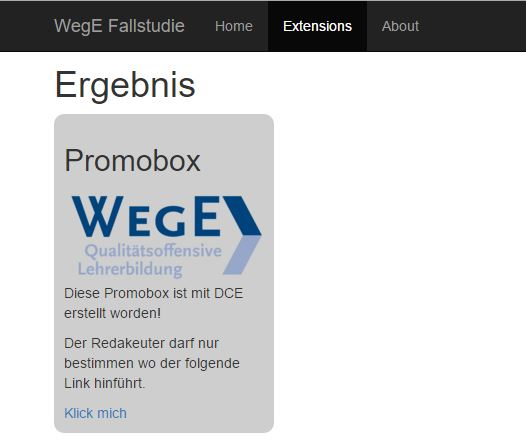
\includegraphics[width=0.5\linewidth]{abb/wegeboxergebnis.jpg}
	\caption[Dynamic Content Elements Extension]{Das Ergebnis der dce Extension}
	\label{fig:forumextension}
\end{figure}

\subsection{Evaluation}


\section{Kalender}

Im Rahmen von WegE w�re eine Kalenderfunktion f�r verschiedene Aspekte interessant. Zum einen lie�en sich so zuk�nftige Termine f�r die �ffentlichkeit anschaulich pr�sentieren. Zum anderen k�nnte ein Kalender Nutzern erlauben sich selbst in bestimmte Beratungstermine einzutragen. Besagte Termine sollen durch Redakteure erstellt werden k�nnen. Eine optimale Extension unterst�tzt also jene Features.

\subsection{M�glichkeiten}

Aufgrund der gesetzten Kriterien ist die einzig sinnvolle Wahl die Kalender Extension Calendar Base. Die Extension ist nicht bescheiden und behauptet alle Features anderer Extensions in eine Extension zu vereinen. Sie wird bereits seit 2006 entwickelt und regelm��ig aktualisiert. Mit �ber 60,000 Downloads ist sie eine der beliebtesten Extensions. Das Manual ist mit �ber 400 Seiten sehr ausf�hrlich. Die Daten des Kalenders sind im iCal Format, was ein Standard f�r Kalenderinformationen ist. Der Kalender kann auch mit externen Kalendern, wie Google Calendar, zusammenarbeiten. Daten k�nnen sowohl im Backend und im Frontend eingetragen werden.

Alternativen zu Calendar Base sind eher rar ges�t und bieten entweder weniger Features oder sind weniger ausgereift. Dies kann aber auch ein Vorteil sein. Sollte man nur bestimmte Features ben�tigen l�sst sich eine �berladung von Features vermeiden. Ein Beispiel hierf�r ist Event Calendar\footnote{https://docs.typo3.org/typo3cms/extensions/gb\_events/}. Es erlaubt einzig die Erstellung und Anzeige einer Liste von anstehenden Events. 

F�r die Anforderungen des WegE Projekt ist Calendar Base am Besten geeignet und wird nun implementiert.

\subsection{Implementation}

\begin{figure}[h]
	\centering
	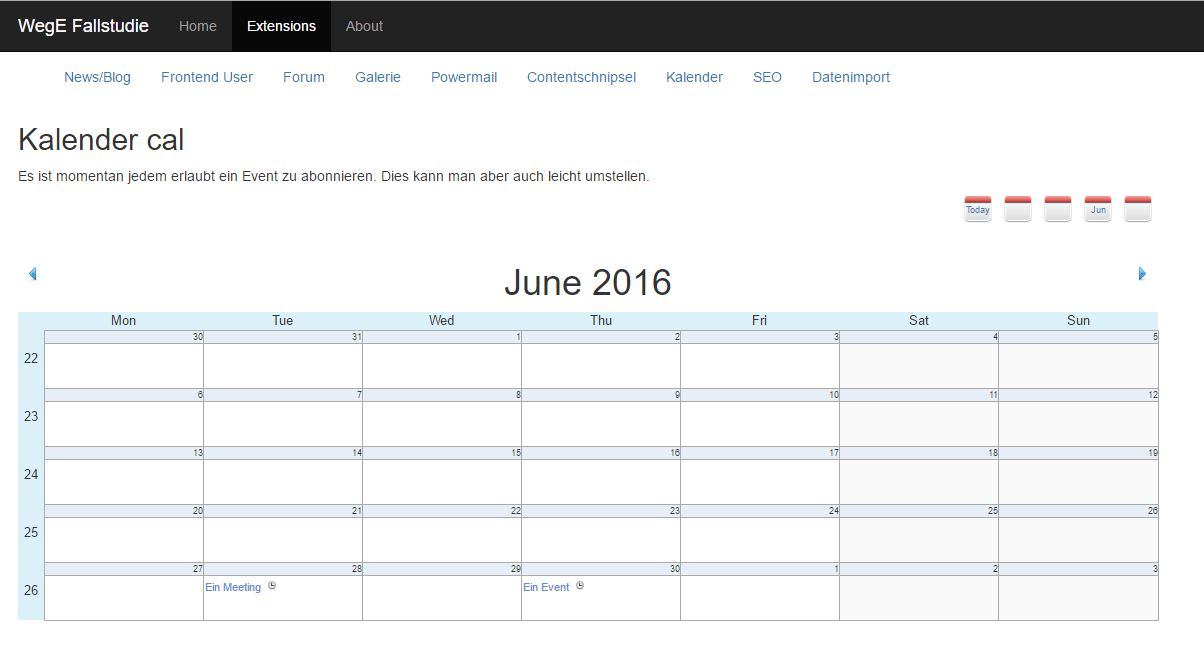
\includegraphics[width=0.75\linewidth]{abb/cal.jpg}
	\caption[Kalender Extension]{Das Ergebnis der cal Extension}
	\label{fig:calextension}
\end{figure}

Wie bei allen Extensions empfiehlt es sich, sich bei der Installation genau an das Manual zu halten, da viele der Extension Installationen einige T�cken bergen. Dar�ber hinaus verl�uft die Installation von cal wie �blich. Die n�tigen Templates werden hinzugef�gt, eine Seite zum Halten der Extension erstellt und konfiguriert. Zuletzt bedarf es einer Zeile Typoscript zur Spezifikation des Sysfolders mit den Terminen.
\begin{verbatim}
options.tx_cal_controller.pageIDForPlugin = {PID}
\end{verbatim}
Es wird eine Seite zur Anzeige angelegt, welche das Plugin einbindet. Hier lassen sich verschiedene Dinge zur Anzeige steuert, es l�sst sich einstellen welche Rechte n�tig sind um Events zu abonnieren und es wird der Ordner spezifiziert, der die Kalendereintr�ge beherbergt.
In der Beispielimplementation k�nnen Events nur im Backend erstellt werden und im Frontend von jedem mittels Email abonniert werden. Handelt es sich bei einem Termin um einen Vortrag kann man so einen �berblick �ber die Anzahl der zu erwartenden G�ste erlangen. Handelt es sich bei dem Termin um eine Einzelsitzung, kann man dem Abonnent anschlie�end weitere Infos an die eingetragene Email senden. 

\subsection{Evaluation}

In der Testumgebung stellte sich das Setup der grundlegenden Features von Calendar Base als relativ einfach heraus. 
Es wird eine monatliche Ansicht angezeigt und auch die erstellten Events tauchen hier auf. Ein Klick auf ein bestimmtes Event zeigt weiter Infos und ein Feld zum Abonnieren des Events via Email an. Lediglich eine Funktion zur Begrenzung von Abonnenten/Teilnehmern ist nicht so einfach zu finden. Wenn ein Nutzer seine Email zu einer Einzelbesprechung angibt und somit diesen Termin f�r sich beansprucht, w�re es praktisch diesen Termin als reserviert anzuzeigen. Dies w�rde eigene Programmierarbeit erfordern. 

\section{Weitere n�tzliche Extensions}

\subsubsection{RealURL}

\subsubsection{SEO}

\subsubsection{YAG - Yet another Gallery}

Will man auf einer Webseite sehr viele Bilder anzeigen, ist es ratsam diese ein wenig zu strukturieren. Das geschieht meist durch die Aufteilung in Galerien und Alben. Dieses sollen dem Betrachter nat�rlich auch ansprechend pr�sentiert werden. Beide dieser Anforderungen werden von der YAG Extension erf�llt. Die Installation ist sehr einfach, zu beachten ist jedoch, dass eine nahtlose Integration nicht trivial ist und einige Anpassungen vorgenommen werden um eine ansprechende Ausgabe zu bekommen. 

\subsubsection{Grid Elements}

\subsubsection{Powermail}

Eine sehr einfach klassifizierbare Extension ist Powermail. Sie erf�llt den Zweck ein Formular anzuzeigen, durch das ein Nutzer der Seite eine Nachricht senden kann ohne in ein externes Mailingprogramm zu wechseln. Dies findet im WegE Projekt als Anlaufstelle eine Verwendung. Die Installation gestaltet sich sehr einfach und alle Aspekte eines solchen Formulars lassen sich bequem �ber das Backend anpassen. Das Formular wird als Plugin in die Seite integriert, bekommt ein erstelltes Formular zugewiesen, erh�lt einen Include im Template und schon ist es betriebsf�hig. Die einzige etwas speziellere Anforderung an diese Extension, die das WegE Projekt haben k�nnte, w�re die M�glichkeit unterschiedlicher Empf�ngeradressen in unterschiedlichen Formularen. Auch das ist kein Problem. Die Wahl auf Powermail fiel aufgrund der Popularit�t und Stabilit�t. Andere �hnliche Extensions unterscheiden sich jedoch kaum.

\begin{figure}
\centering
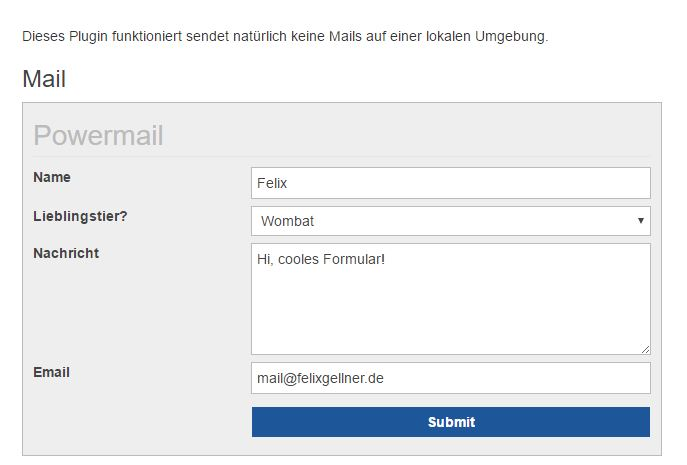
\includegraphics[width=0.5\linewidth]{abb/powermail.jpg}
\caption[Powermail Extension]{Ein Formular erstellt mit Powermail}
\label{fig:powermail}
\end{figure}


\section{Wartung und Sicherheit}



\chapter{Validierung der Requirements basierend auf der Implementation}
Nachdem die Umsetzung der Liste von Requirements aus Kapitel \ref{kap-projektanalyse} beendet ist, k�nnen diese Requirements validiert werden. Die Validierung geschieht in diesem meist anhand der Kriterien Korrektheit,  Machbarkeit und Notwendigkeit. Nach der prototypischen Implementation der WegE Requirements ist vor Allem die Validierung der Machbarkeit interessant.\\
Korrektheit betrachtet die Formulierung des Requirements und ob dieses vielleicht falsch gestellt wurde.
Machbarkeit untersucht mit Hilfe des Wissens �ber die Technologie, ob die gew�hlten Requirements tats�chlich umgesetzt werden k�nnen. Dabei sollten Budget und Zeit mit in Betracht gezogen werden.
Notwendigkeit untersucht ob einige der Requirements eventuell nicht umgesetzt werden m�ssen. \cite{Sommerville2007}
\paragraph{Validierung der untersuchten WegE Requirements}
\begin{itemize}
	\item \textbf{Statische Informationen}\\
	Dieser Punkt klingt trivial, doch manche Systeme erf�llen dieses Requirement besser als andere. In Typo3 lassen sich statische Webseiten leicht erstellen und kompromisslos anzeigen. Lediglich das Backend k�nnte f�r Redakteure zu Beginn etwas einsch�chternd sein, weshalb eventuell etwas anf�ngliche Unterst�tzung aus der IT Abteilung n�tig ist. Die Machbarkeit ist dennoch gegeben. Die Notwendigkeit daf�r ist auch sehr hoch, da die �ffentlichkeit in das WegE Projekt mit einbezogen werden soll. 
	
	\item \textbf{Newsfeed}\\
	Die Implementation eines Newsfeed stellte sich als recht einfach heraus. Die news Extension l�uft stabil und l�sst sich nach Bedarf sogar mit vielen weiteren Extensions erweitern/verbinden. F�r einen einfachen Newsfeed ist die Machbarkeit absolut gegeben. Ein Newsfeed hat dieselbe Aufgabe, wie statische Informationen, doch bietet stetige aktuelle Informationen strukturierter an, als solche. Wieder geht es darum Informationen nach au�en zu tragen, was die Notwendigkeit hoch einstuft.
	
	\item \textbf{Blogs}\\
	Der Blog �hnelt dem Newsfeed, zumal sich dieser im Test mit derselben Extension realisieren lie�. Doch bietet ein Blog deutlich mehr Umfang als ein Newsfeed. Die Aufgabe ist einerseits wieder Informationen zu teilen. Andererseits soll ein Blog auch Aufmerksamkeit auf ein Produkt lenken. Die Notwendigkeit von Aufmerksamkeit ist sehr hoch, was einen Blog wichtig macht. Allerdings sollte beachtet werden, dass ein Blog regelm��ig mit Updates versorgt werden muss, um gew�nschte Effekte zu erzielen und diese Updates sind Arbeit. Somit ist die technische Machbarkeit voll gegeben, doch die allgemeine Machbarkeit k�nnte etwas niedriger sein. 
	
	\item \textbf{Redakteure}\\
	Redakteure werden im WegE Projekt von jeder Abteilung eingesetzt, um �ber Neuigkeiten zu berichten. Besonders wenn ein News Feed oder ein Blog zum Einsatz kommt sind Redakteure unabdingbar. Typo3 erlaubt das Erstellen von Konten f�r viele Nutzer, deren Rechte individuell angepasst werden k�nnen. Um den Redakteuren ihre Arbeit leichter zu machen, lassen sich eigene Contentelemente anlegen und unn�tige Bereiche des Backend verstecken. Die Machbarkeit ist gegeben, Notwendigkeit ist mit der Entwicklung eines Blogs oder �hnlichem, gegeben.
	
	\item \textbf{Forum}\\
	Das Forum ist ein Weg f�r Besucher einer Webseite in n�heren Kontakt zu treten und Diskussionen zu f�hren. In der Implementation hat sich gezeigt, dass ein Forum mit Typo3 machbar ist, doch dessen Anpassung einiges an Arbeit fordert. Die Notwendigkeit ist nach dem aktuellen Stand der WegE Plattform nicht eindeutig gegeben. Um ein sinnvolles Forum aufzubauen, wird eine kritische Masse an Nutzern ben�tigt, die miteinander diskutieren k�nnen und diese ist bei dem speziellen Thema der WegE eventuell problematisch. Dazu umfassen die Ziele der WegE Plattform momentan nicht den Aufbau einer Community. Sollte sich das �ndern, w�rde das Forum eine sehr gute Option darstellen. Solange ist die Notwendigkeit eher gering einzusch�tzen.
	
	\item \textbf{Registrierung}\\
	Die Registrierung von Frontend Nutzern ist vor Allem dann interessant, wenn das Forum implementiert wird. Die Extension zu den Frontend Usern l�sst sich sogar leicht mit der Forum Extension verbinden. Aber auch andere Anwendungsbeispiele sind m�glich. So k�nnten zum Beispiel nur registrierte Nutzer Eintr�ge in den Kalender t�tigen oder auf bestimmte Seiten mit Downloads zu neuen Dissertationen. Dank einer exzellenten Extension ist die Registrierung leicht machbar, h�ngt aber auch von der Anzahl der Anwendungsszenarien ab. Die Notwendigkeit ist sehr hoch, sobald ein Forum implementiert wird oder Zugriffsrechte auf bestimmte Downloads beschr�nkt werden soll. Ohne solche Features ist diese Registrierung nicht notwendig.
	
	
	\item \textbf{Forschungsergebnisse teilen}\\
	Das Teilen neuer Forschungsergebnisse ist einer der Hauptziele der WegE Plattform und somit absolut notwendig. Im Test wird aufgezeigt, dass dies �ber verschiedene Ans�tze m�glich ist, nicht zuletzt �ber Typo3 selbst. Daraus folgt eine sehr hohe Machbarkeit.
	
	\item \textbf{Mail Formular}\\
	Mit dem Mail Formular l�sst sich ohne Umwege in ein E-Mail Programm eine Nachricht an die Seitenbetreiber senden. Dieses Formular erleichtert die Kontaktaufnahme sehr, weshalb die Notwendigkeit relativ hoch ist. Dazu kommt eine sehr hohe Machbarkeit, durch die unkomplizierte powermail Extension.
	
	\item \textbf{Kalender}\\
	Die Anwendungen f�r den Kalender sind Informationen zu teilen und Events abonnieren zu k�nnen. Die Extension im Test bietet das und vieles mehr. Die Implementation stellt sich als recht aufw�ndig heraus. Die Machbarkeit f�r die oberen zwei Punkte, die auch im Test umgesetzt wurden, ist voll gegeben. Sollen weitere Features des Kalenders implementiert werden, kann der Aufwand steigen. Eine �bersicht �ber kommende Termine ist auf die eine oder andere Weise sehr w�nschenswert, womit die Notwendigkeit des Kalenders relativ hoch ist.
	
	\item \textbf{Search Engine Optimization}\\
	Je h�her eine Seite auf einer Suchmaschine gelistet ist, desto besser. Typo3 sorgt an sich schon f�r einige Optimierungen f�r Suchmaschinen. Viele Felder f�r meta-tags werden den Redakteuren angeboten. Einige Extensions erweitern dies Funktionalit�ten noch ein wenig, der Gro�teil muss jedoch manuell f�r jede Seite gemacht werden. Diese kleinen Anpassungen bedeuten etwas mehr Arbeit sind aber absolut machbar. Die Notwendigkeit von SEO ist allgemein sehr hoch, doch die Notwendigkeit zus�tzlicher Extensions ist eher mittelm��ig, da die Effektivit�t dieser eher gering bleibt.
	
\end{itemize}


           
% Weitere Kapitel ...
\chapter{Zusammenfassung} 
\label{kap-zusammenfassung}%

In dieser Arbeit wurde behandelt, wie ein web-basiertes Projekt richtig angegangen werden sollte. Es wurde gezeigt, wie sich der Prozess der Softwareentwicklung, trotz sehr unterschiedlicher Modelle immer in f�nf Phasen einteilen l�sst. Analyse, Entwurf, Implementierung, Testen und Wartung. Alle Schritte wurden, am Beispiel der WegE Plattform der Universit�t Bamberg, welches aktuell umgesetzt wird, konkretisiert. Zu Beginn eines Projekts spielt das Requirements Engineering eine entscheidende Rolle, bei welchem alle n�tigen Anforderungen eines Projekts sammelt. Sind bei einigen Requirements Unklarheiten �ber Machbarkeit dieser, ist es sinnvoll diese prototypisch zu testen und die Ergebnisse dessen zu validieren. Eine solche Liste mit unklaren Requirements wurde in dieser Arbeit getestet. Vor dem Test wurde erkl�rt, wie passende Technologien, genauer CMS, f�r ein Projekt bestimmt werden. Neben technischen Daten spielen hier auch Budget und Vorwissen eine gro�e Rolle. Diese Kriterien wurden an drei ausgew�hlten CMS untersucht. F�r das WegE Projekt fiel die Wahl auf Typo3, welches ausf�hrlich vorgestellt wird um dann die zuvor ausgew�hlten Requirements zu implementieren und zu testen. Aus Gr�nden der Effizienz wurden dabe vor Allem die M�glichkeiten von Extensions untersucht. Nach der Implementierung lie� sich die Validierung dieser Anforderungen durchf�hren und die erhaltenen Ergebnisse k�nnen in die weitere Planung des WegE Projekt flie�en.

\section{Erkenntnisse}

Typo3 ist ein flexibles und sehr m�chtiges Web Content Management System. Als jemand mit fundierten Kenntnissen in der Webentwicklung und dem WCMS Worpress, war Ich dennoch von der Gr��e erschlagen. Typo3 ist nicht f�r Projekte geeignet, die alleine bew�ltigt werden k�nnen. F�r gro�e Projekte ist es jedoch eine fantastische Wahl und je mehr ich in Typo3 arbeitete, desto klarer wurden die M�glichkeiten und Vorz�ge. Durch die steile Lernkurve von Typo3 sind diese f�r Anf�nger n�mlich nicht unbedingt ersichtlich. 
Einer der leicht ersichtlichen Vorteile ist das Extension Repository. Sich durch wenige Klicks neue Funktionalit�t ins System zu laden ist �berzeugend. Die Auswahl und Qualit�t der Extensions ist �berwiegend gut. Allerdings sind viele der Extensions keine komplette Out-of-the-box-L�sung und ben�tigen eine Portion Eigeninitiative. Vor Allem wenn es an spezielle Anpassungen geht. Dies ist f�r schnelle, kleine Projekte von Nachteil, f�r gro�e Projekte gewinnt man dadurch mehr Kontrolle �ber die Extensions. 
Beim Kapitel zur Projektanalyse wurde sehr deutlich welche Vorteile gut Planung haben kann. Doch auch einige negative Aspekte fielen auf. Bei sehr vielen Konzepten des Software Engineering handelt es sich um Richtlinien, welche nur von Vorteil sind, wenn sie an der richtigen Stelle angewendet werden. So fiel mir bei der Recherche dazu auf, dass auch zu viel geplant werden kann und die Planung damit dem Projekt sogar schaden kann. Ist der Ausgang des Projekts jedoch kritisch und die Projektdomain neu, sollte definitiv nicht auf gutes Software Engineering verzichtet werden. 


\section{Ausblick auf die Zukunft von CMS Entwicklung und der WegE Plattform}

Das Erstellen von Web Plattformen ist so leicht wie noch nie. Der Andrang auf das Internet und Webseiten aller Art, brachte auch die Tools f�r Entwickler voran. Durch diese Evolution stieg auch die Komplexit�t und Anforderungen an moderne Webseiten, weshalb die Entwicklung dieser nach mehr Planung verlangt, als je zuvor. 
Typo3 entwickelt stets an neuen Versionen. Die n�chste Version, Nummer 8, kommt mit einigen sehr n�tzlichen Ver�nderungen. So werden Anliegen wie Cloud Integration, PHP7 Support, einem integrierten Form Builder und verbesserten Tools f�r Redakteure.\footnote{https://typo3.org/typo3-cms/roadmap/}
Der Web Development Sektor ver�ndert sich allgemein immer noch extrem schnell, weshalb auch schnell Unsicherheiten auftreten, ob es sich lohnt auf eine bestimmte Technologie zu setzen. Doch die Typo3 Community ist sehr stark und vor Allem die �nderungen in Version 7 und 8 bringen Typo3 als Wahl f�r WCMS wieder weit nach vorne. Ich hoffe, dass diese Entwicklung des Web Development stetig weitergeht und Entwickler sich so mehr aufs Wesentliche konzentrieren und bei der Entwicklung weiterhin Spa� haben k�nnen.   

\appendix
\chapter{Anhang - Bootstrap Fluidtemplate}


\paragraph{index.html}

In der Index.html wird das Men� folgenderma�en eingebunden.
\begin{verbatim}
	[...]
	<div id="navbar" class="collapse navbar-collapse">
	  <f:cObject typoscriptObjectPath="lib.mainmenu" />
	</div>
	[...]
\end{verbatim}

Der restliche Content wird f�r die Zwecke dieser Arbeit nicht speziell behandelt. Folgender Code in der index.html reicht aus.
\begin{verbatim}
<f:format.raw>{content}</f:format.raw>
\end{verbatim}


\paragraph{setup.ts}

Die setup.ts f�r das simple Bootstrap Men�.
\begin{verbatim}
	config.contentObjectExceptionHandler = 0
	# Main Menu
	lib.mainmenu = HMENU
	lib.mainmenu{
	 entryLevel = 0
	 1 = TMENU
	 1{
 	  wrap = <ul class="nav navbar-nav"> | </ul>
	  noBlur = 1
	  NO = 1
	  NO{
	   wrapItemAndSub = <li> | </li>
	   stdWrap.htmlSpecialChars = 1
	   ATagTitle.field = title
	  }
	  ACT <.NO
	  ACT{
	   wrapItemAndSub = <li class="active"> | </li>
	  }
	 }
	}
	#Submenu, 2nd layer
	lib.submenu = HMENU
	lib.submenu{
	 entryLevel = 1
	 1 = TMENU
	 1{
	  wrap = <ul class="nav navbar-nav"> | </ul>
	  noBlur = 1
	  NO = 1
	  NO{
	   wrapItemAndSub = <li> | </li>
	   stdWrap.htmlSpecialChars = 1
	   ATagTitle.field = title
	  }
	  ACT <.NO
	  ACT{
	   wrapItemAndSub = <li class="active"> | </li>
	  }
	 }
	}
	
	page = PAGE
	page{
	 includeCSS.bootstrap = fileadmin/Template_WegE/bootstrap/css/bootstrap.min.css
	 includeCSS.style = fileadmin/Template_WegE/bootstrap/css/style.css
	 includeJSFooter.jquery = fileadmin/Template_WegE/bootstrap/js/jquery-2.2.3.min.js
	 includeJSFooter.bootstrapjs = fileadmin/Template_WegE/bootstrap/js/bootstrap.min.js
	
	 10 = FLUIDTEMPLATE
	 10{
	  file = fileadmin/Template_WegE/index.html
	  layoutRootPath = fileadmin/Template_WegE/layouts/
	  partialRootPath = fileadmin/Template_WegE/partials/
	
	  variables{
	   siteName = TEXT
	   siteName.value = WegE Fallstudie
	
	   content < styles.content.get
	  }
	 }
	}
\end{verbatim}


%Abbildungsverzeichnis
\addcontentsline{toc}{chapter}{Abbildungsverzeichnis}
\listoffigures

%Tabellenverzeichnis
\addcontentsline{toc}{chapter}{Tabellenverzeichnis} \listoftables

% Literaturverzeichnis
\addcontentsline{toc}{chapter}{\bibname}
\bibliography{bibl}

\newpage
\pagestyle{empty}
Ich erkl�re hiermit gem�� � 27 Abs. 2 APO, dass ich die
vorstehende Diplomarbeit selbstst�ndig verfasst und keine anderen
als die angegebenen Quellen und Hilfsmittel benutzt habe.
\vspace{1cm}

Bamberg, 31.05.2005\hspace{5cm}

\end{document}
